\chapter{Risultati}
\label{cap:risultati}

Il capitolo segue le quattro fasi definite in \cref{sec:disegno-fasi}: le prime tre
fasi caratterizzano i backend CUDA con un solo processo MPI, mentre la quarta
fase porta le configurazioni ottenute nell'applicazione distribuita completa, dove più
rank condividono l'unica GPU del nodo.

\section{Fase 1 - Configurazione dei backend CUDA}
\label{sec:ris-fase1}

Tutte le misure di questa sezione sono prese a $M = N = \num{16384}$, doppia
precisione, $P = 1$.

\subsection{Campagna 1.1 - Dimensione del blocco}
\label{sec:ris-block}

La \cref{tab:ris-block-perdite} riporta, per ciascun kernel e ciascun valore di
\code{BLOCK}, le due statistiche di perdita definite nella
\cref{eq:perdita-max}: quanto quella dimensione di blocco perde, in media e nel
caso peggiore, rispetto al miglior blocco \emph{per lo stesso} $k$.

\begin{table}[H]
\centering
\footnotesize
\caption{Campagna 1.1: perdita rispetto al miglior \code{BLOCK} per lo stesso
$k$, in percentuale. In grassetto il valore selezionato per ciascun kernel.}
\label{tab:ris-block-perdite}
\begin{tabular}{@{}rrrrr@{}}
\toprule
& \multicolumn{2}{c}{\kernelname{cuda\_naive}}
& \multicolumn{2}{c}{\kernelname{cuda\_warp}} \\
\cmidrule(lr){2-3}\cmidrule(lr){4-5}
\code{BLOCK} & media & max & media & max \\
\midrule
64   & 1,13  & 3,85  & 0,41 & 1,32 \\
128  & \textbf{0,92} & \textbf{1,69} & \textbf{0,42} & \textbf{0,74} \\
192  & 3,55  & 8,21  & 0,98 & 1,99 \\
256  & 1,09  & 4,56  & 1,19 & 3,95 \\
384  & 3,84  & 9,71  & 1,27 & 1,78 \\
512  & 5,64  & 10,23 & 3,17 & 5,89 \\
1024 & 10,86 & 23,29 & \multicolumn{2}{c}{\scriptsize\itshape\shortstack{lancio fallito\\per $k = 20$ e $k = 32$}} \\
\bottomrule
\end{tabular}
\end{table}

I valori selezionati sono quindi $\code{BLOCK} = 128$ per
\kernelname{cuda\_naive} e \kernelname{cuda\_warp}, $\code{BLOCK} = 256$ per
\kernelname{cuda\_warp\_smem}. Le prestazioni assolute corrispondenti sono
riportate in \cref{tab:ris-block-assolute}.

\begin{table}[H]
\centering
\footnotesize
\caption{Campagna 1.1: \code{gflops\_kernel} al \code{BLOCK} selezionato.}
\label{tab:ris-block-assolute}
\begin{tabular}{@{}lrrrrr@{}}
\toprule
\textbf{Backend} & $k=3$ & $k=6$ & $k=8$ & $k=20$ & $k=32$ \\
\midrule
\kernelname{cuda\_naive} (\code{BLOCK}=128)      & 149,3 & 308,7 & 337,3 & 345,6 & 350,3 \\
\kernelname{cuda\_warp} (\code{BLOCK}=128)       & 300,3 & 351,4 & 350,3 & 351,4 & 352,5 \\
\bottomrule
\end{tabular}
\end{table}

\begin{figure}[H]
\centering
\begin{subfigure}{\linewidth}
  \centering
  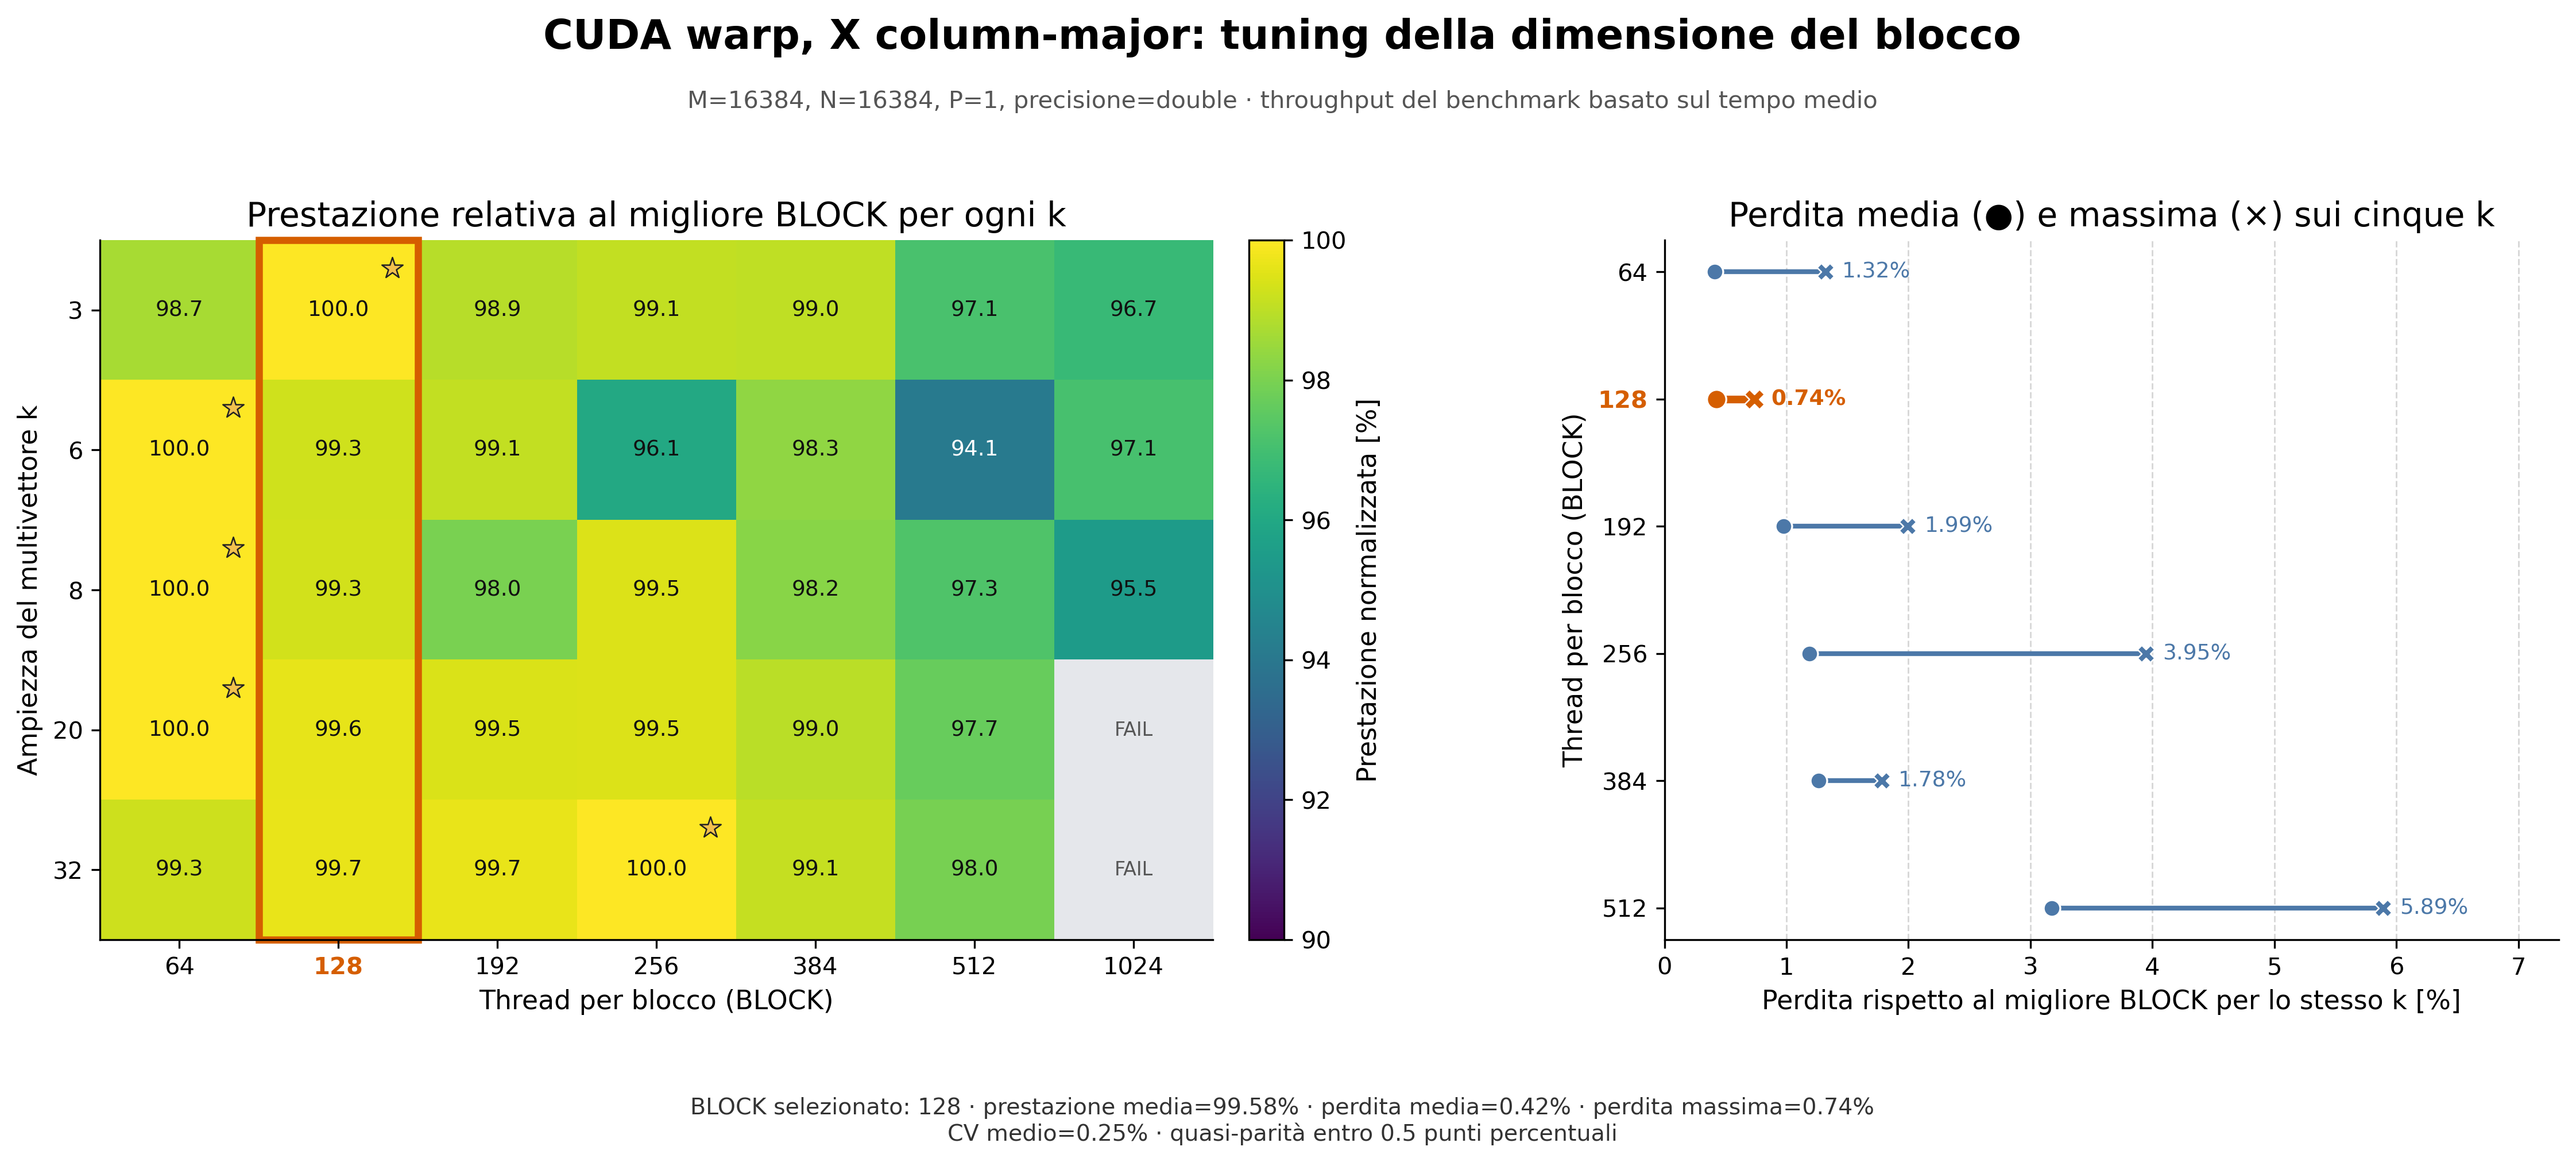
\includegraphics[width=\linewidth]{img/fase1/campagna_VAS_block_k_tuning/campagna_VAS_block_k_tuning_summary_cuda_warp_xcolumn.png}
  \caption{\kernelname{cuda\_warp}, $X$ column-major.}
\end{subfigure}

\caption{Campagna 1.1: prestazione normalizzata per $(\code{BLOCK}, k)$ a
sinistra, perdita media e massima sui cinque $k$ a destra. Le celle
\code{FAIL} sono i lanci non riusciti a \code{BLOCK}$=1024$.}
\label{fig:ris-block}
\end{figure}

\begin{figure}[H]
\centering
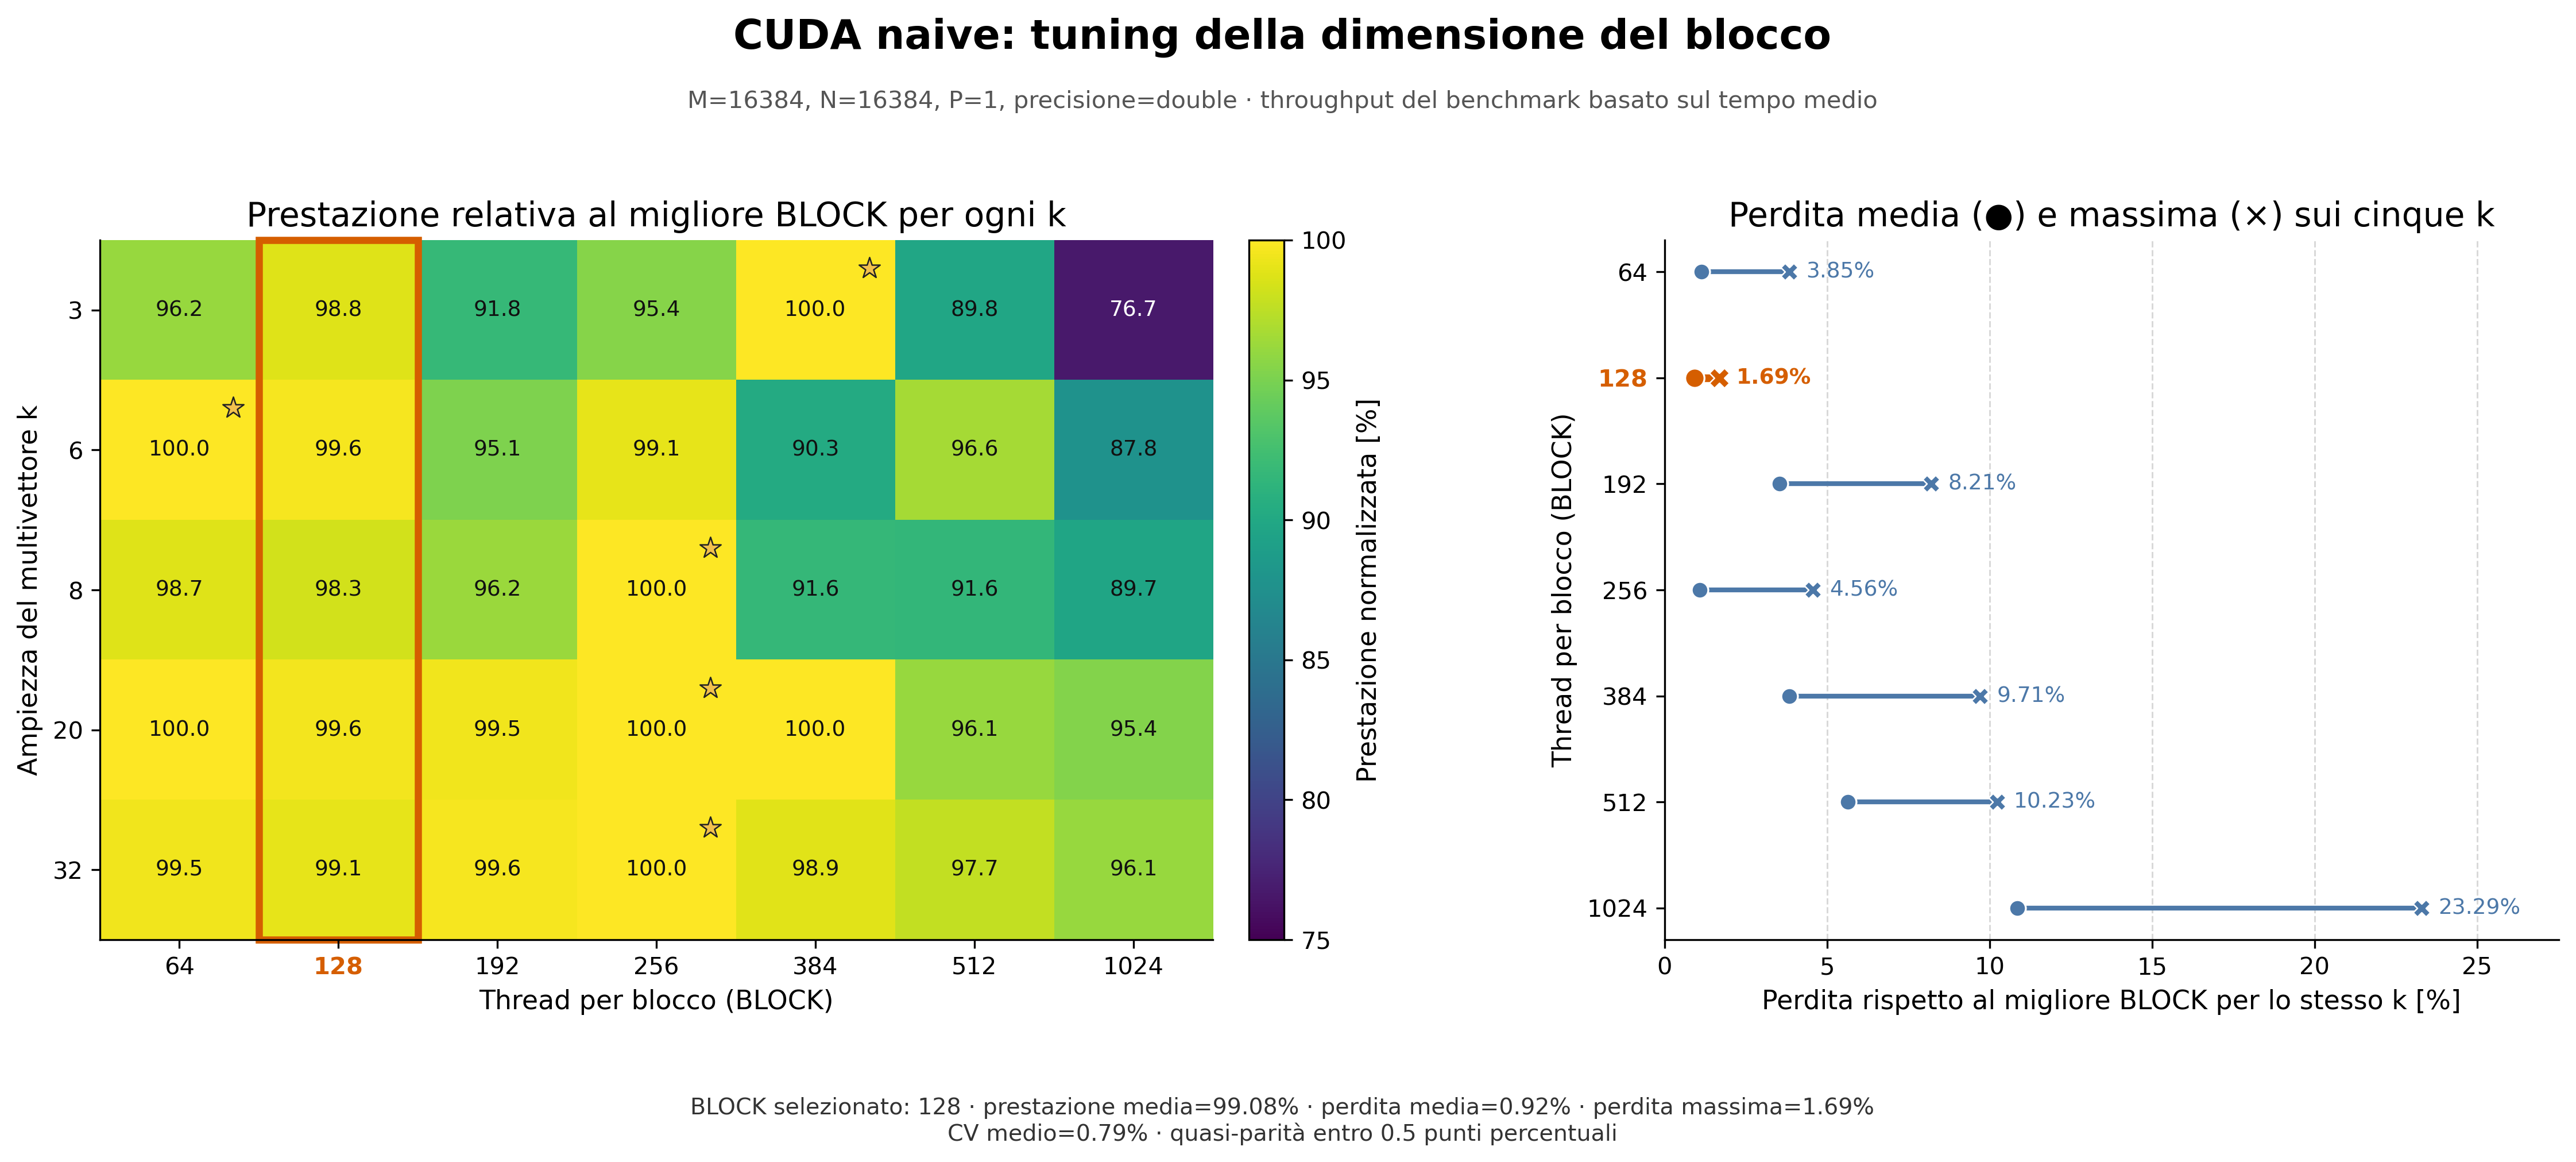
\includegraphics[width=\linewidth]{img/fase1/campagna_VAS_block_k_tuning/campagna_VAS_block_k_tuning_summary_cuda_naive.png}
\caption{Campagna 1.1: stessa lettura per \kernelname{cuda\_naive}, l'unico
kernel che completa anche a \code{BLOCK}$=1024$.}
\label{fig:ris-block-naive}
\end{figure}

\subsubsection*{Lettura}

\textbf{La sensibilità a \code{BLOCK} dipende dalla struttura del kernel.}

\kernelname{cuda\_warp} è il backend meno sensibile nell'intervallo delle
configurazioni valide. Fra 64 e 384 thread per blocco le prestazioni rimangono
vicine all'ottimo e il valore selezionato, \code{BLOCK}=128, limita la perdita
massima allo $0{,}74\%$. Il risultato è coerente con la mappatura
warp-per-row: il lavoro associato a una riga di $Y$ è già definito alla
granularità del warp, per cui modificare la dimensione del blocco cambia
principalmente quanti warp vengono raggruppati nello stesso blocco, senza
modificare il lavoro assegnato a ciascuno di essi.

\textbf{Non emerge una regola semplice basata sulla sola dimensione del
blocco.}

Per \kernelname{cuda\_naive}, ad esempio, le configurazioni
\code{BLOCK}=192 e \code{BLOCK}=384 risultano peggiori di 128 e 256, ma lo
stesso andamento non si ripete in modo uniforme sugli altri kernel.
Analogamente, \code{BLOCK}=512 produce per \kernelname{cuda\_warp} una perdita
maggiore rispetto a blocchi più piccoli. Il numero di thread per blocco non è
quindi sufficiente, da solo, a spiegare le differenze osservate. Alla
geometria del lancio si aggiungono infatti il consumo di registri per thread.

\textbf{I fallimenti a \code{BLOCK}=1024 costituiscono un ulteriore limite
della configurazione.}

Con 1024 thread per blocco,
\kernelname{cuda\_warp}  non completa
l'esecuzione per $k=20$ e $k=32$, mentre \kernelname{cuda\_naive} continua a
essere eseguibile. La differenza è coerente con la diversa pressione sui
registri: il kernel naive mantiene un solo accumulatore per thread, mentre
nelle istanze specializzate dei due kernel warp ogni lane mantiene un vettore
di $k$ accumulatori.

\textbf{Esito della campagna.}
Il criterio di robustezza porta a selezionare \code{BLOCK}=128 per
\kernelname{cuda\_naive} e per \kernelname{cuda\_warp}. In entrambi i casi la
configurazione scelta rimane molto vicina al miglior valore specifico per
ciascun $k$, evitando di ottimizzare il kernel per un solo punto della
traccia.

\subsection{Campagna 1.2 - Layout in memoria di $X$}
\label{sec:ris-layout}

\begin{table}[H]
\centering
\footnotesize
\caption{Campagna 1.2: \kernelname{cuda\_warp} con $X$ row-major e
column-major, \code{BLOCK}$=128$. L'ultima colonna è il costo della conversione
di $X$, che è preprocessing e non entra in $T$.}
\label{tab:ris-layout}
\begin{tabular}{@{}rrrrrr@{}}
\toprule
$k$ & row-major & column-major & speedup & $t_{\text{kernel}}$ row & $t_{\text{convert}}$ \\
    & [GFLOPS] & [GFLOPS] & col/row & [\si{\milli\second}] & [\si{\milli\second}] \\
\midrule
3  & 297,3 & 300,3 & 1,01 & 5,4   & 0,26 \\
6  & 352,0 & 351,4 & 1,00 & 9,2   & 0,57 \\
8  & 182,6 & 350,3 & 1,92 & 23,5  & 0,88 \\
20 & 174,1 & 351,4 & 2,02 & 61,7  & 2,43 \\
32 & 92,2  & 352,5 & 3,82 & 186,4 & 3,32 \\
\bottomrule
\end{tabular}
\end{table}

\begin{figure}[H]
\centering
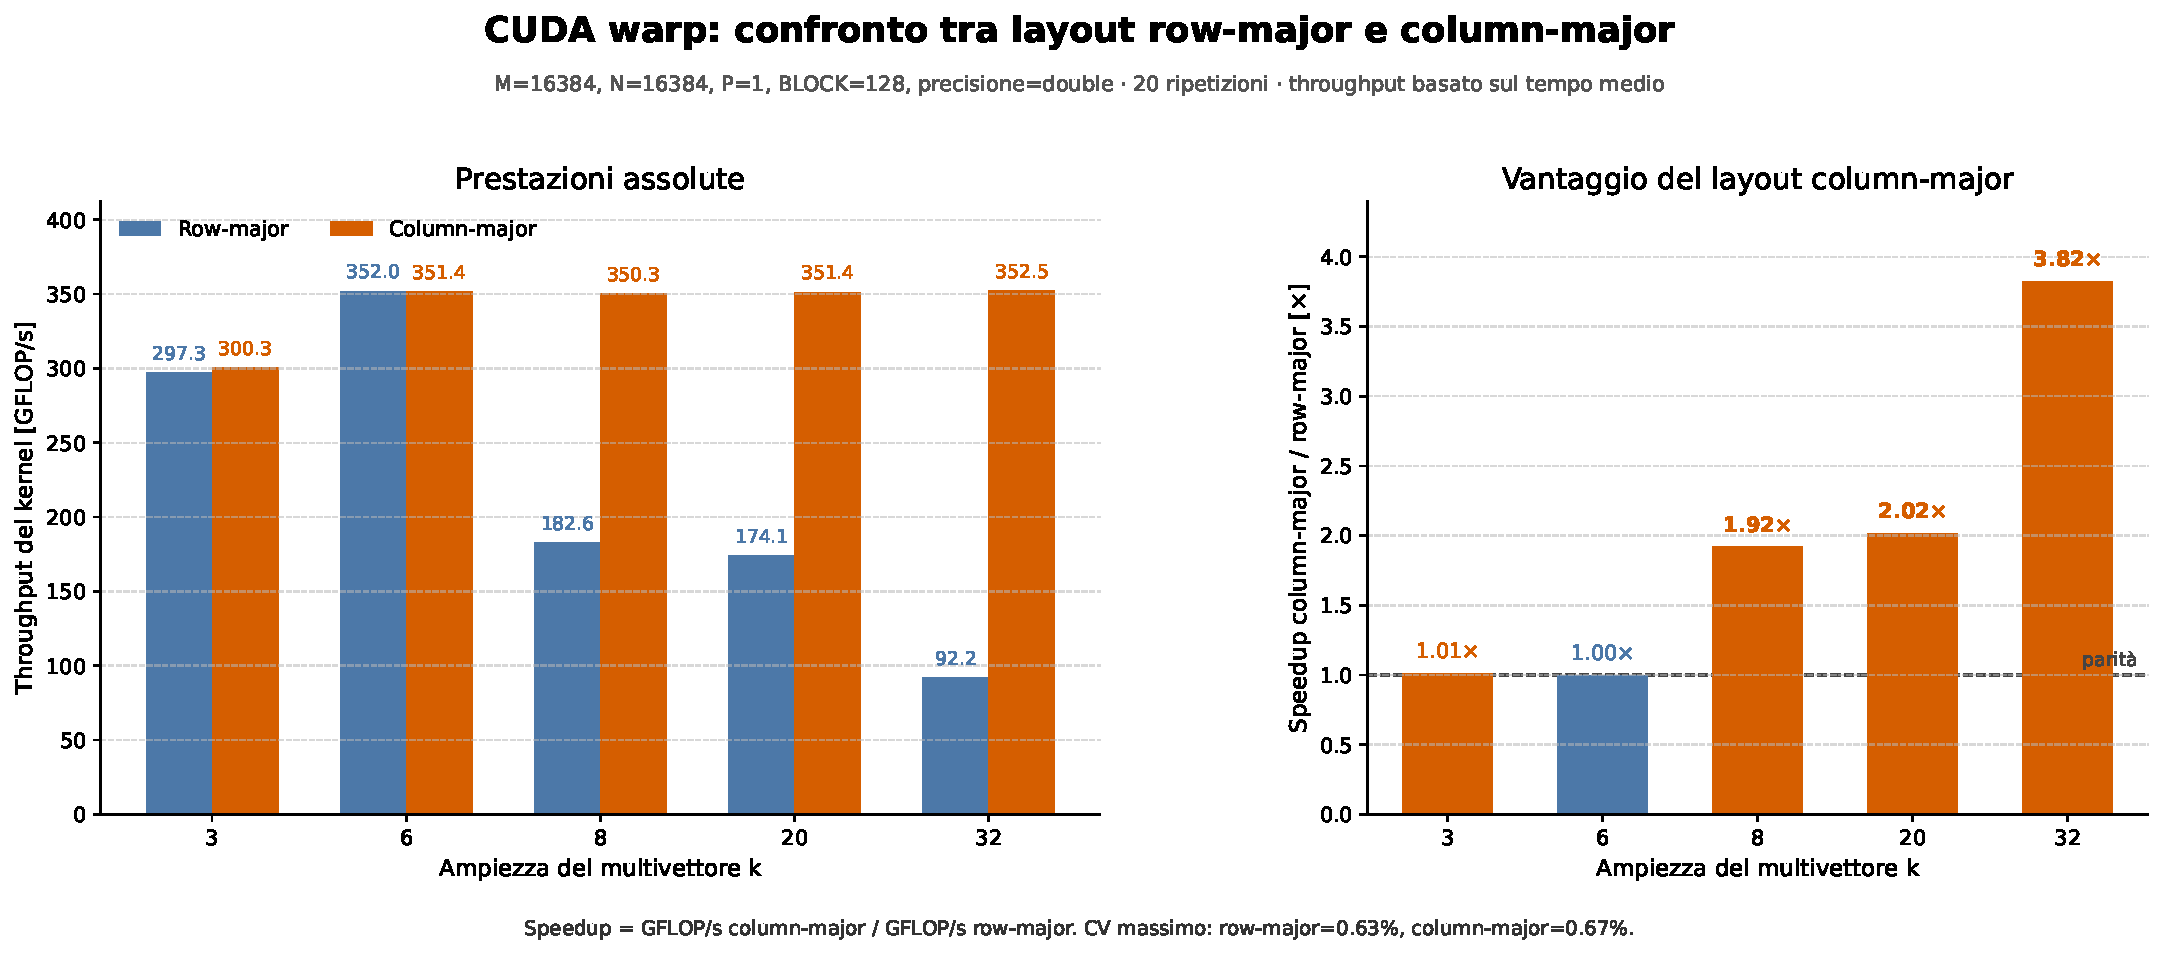
\includegraphics[width=\linewidth]{img/fase1/campagna_VAS_2_row_major/campagna_VAS_2_layout_comparison}
\caption{Campagna 1.2: prestazioni assolute (sinistra) e vantaggio del layout
column-major (destra). CV massimo: $0{,}63\%$ row-major, $0{,}67\%$
column-major.}
\label{fig:ris-layout}
\end{figure}

\subsubsection*{Lettura}

\textbf{L'effetto del layout emerge a partire da $k=8$.}

Per $k=3$ e $k=6$ le due varianti hanno prestazioni molto simili:
lo speedup del layout column-major vale rispettivamente $1{,}01\times$ e
$1{,}00\times$, con coefficienti di variazione inferiori allo $0{,}7\%$.
In questa regione l'eventuale vantaggio è quindi dello stesso ordine della
dispersione delle misure e non è sufficientemente marcato da attribuirgli un
significato prestazionale.

A partire da $k=8$ il comportamento cambia nettamente: il layout
column-major raggiunge uno speedup di $1{,}92\times$, che sale a
$2{,}02\times$ per $k=20$ e a $3{,}82\times$ per $k=32$.

Il vantaggio cresce
quindi all'aumentare della larghezza del multivettore e rende il layout
column-major la scelta naturale per \kernelname{cuda\_warp} nelle campagne
successive.

\textbf{L'andamento è coerente con il pattern di accesso previsto dal kernel.}

In \kernelname{cuda\_warp} lane consecutive elaborano valori consecutivi
dell'indice $j$. Per una colonna $c$ fissata, con $X$ row-major esse richiedono

\[
X[j_0][c],\;
X[j_0+1][c],\;
\ldots,\;
X[j_0+31][c],
\]

che nel buffer sono separati da uno stride di $k$ elementi. All'aumentare di
$k$ gli indirizzi richiesti dalle lane dello stesso warp risultano quindi
sempre più distanti, rendendo meno favorevole il raggruppamento degli accessi
alla global memory.

Con $X$ column-major gli stessi elementi sono invece \emph{consecutivi} in memoria.
Il kernel mantiene invariata la propria mappatura warp-per-row, ma le richieste
delle lane possono essere servite mediante accessi molto più compatti. La
crescita del vantaggio con $k$ è quindi coerente con l'ipotesi che il layout
row-major penalizzi progressivamente il percorso di lettura di $X$.

I risultati mostrano che la differenza fra i layout diventa rilevante proprio quando
aumenta lo stride fra gli elementi letti simultaneamente dalle lane.

\textbf{Il confronto chiarisce anche il ruolo della shared memory.}

\kernelname{cuda\_warp\_smem} mantiene $X$ nel layout row-major, ma evita che
il pattern strided del kernel \code{cuda_warp} venga ripetuto direttamente sulla global
memory. Il tile di $X$ viene prima caricato cooperativamente dai thread del
blocco, utilizzando accessi globali contigui, e viene successivamente
consumato dalla shared memory secondo la solita mappatura warp-per-row.

Le due varianti affrontano quindi lo stesso limite del percorso row-major con
strategie differenti: \kernelname{cuda\_warp} modifica la rappresentazione
fisica di $X$, mentre \kernelname{cuda\_warp\_smem} mantiene il layout
originario e modifica il percorso attraverso cui i dati raggiungono le lane.
Il confronto conclusivo della Fase~1 permette di valutare quale delle due
strategie risulti più conveniente nel regime studiato.


\subsection{Campagna 1.3 - Granularità del tile}
\label{sec:ris-granularita}

\begin{table}[H]
\centering
\footnotesize
\caption{Campagna 1.3: prestazione normalizzata di \kernelname{cuda\_warp\_smem}
per ogni coppia $(\code{BLOCK}, g)$, in percentuale dell'ottimo per lo stesso
$k$. Media sui cinque $k$ e caso peggiore. In grassetto la coppia selezionata.}
\label{tab:ris-granularita}
\begin{tabular}{@{}rrrrrrrrr@{}}
\toprule
& \multicolumn{2}{c}{$g = 1$} & \multicolumn{2}{c}{$g = 8$}
& \multicolumn{2}{c}{$g = 16$} & \multicolumn{2}{c}{$g = 32$} \\
\cmidrule(lr){2-3}\cmidrule(lr){4-5}\cmidrule(lr){6-7}\cmidrule(lr){8-9}
\code{BLOCK} & media & peggiore & media & peggiore & media & peggiore & media & peggiore \\
\midrule
64  & 83,6 & 54,7 & 82,7 & 53,8 & 77,4 & 46,2 & 86,8 & 61,0 \\
128 & 88,0 & 51,3 & 84,3 & 50,5 & 82,2 & 50,4 & 98,7 & 97,1 \\
192 & 79,0 & 67,4 & 76,5 & 66,4 & 87,7 & 71,9 & 94,9 & 81,1 \\
256 & 85,0 & 65,5 & 98,1 & 94,4 & 96,7 & 87,8 & \textbf{99,0} & \textbf{98,5} \\
384 & 89,1 & 80,0 & 89,9 & 78,6 & 89,5 & 76,0 & 90,5 & 80,2 \\
512 & 91,9 & 82,8 & 92,3 & 90,7 & 90,6 & 86,0 & 92,2 & 89,7 \\
\bottomrule
\end{tabular}
\end{table}

\begin{figure}[H]
\centering
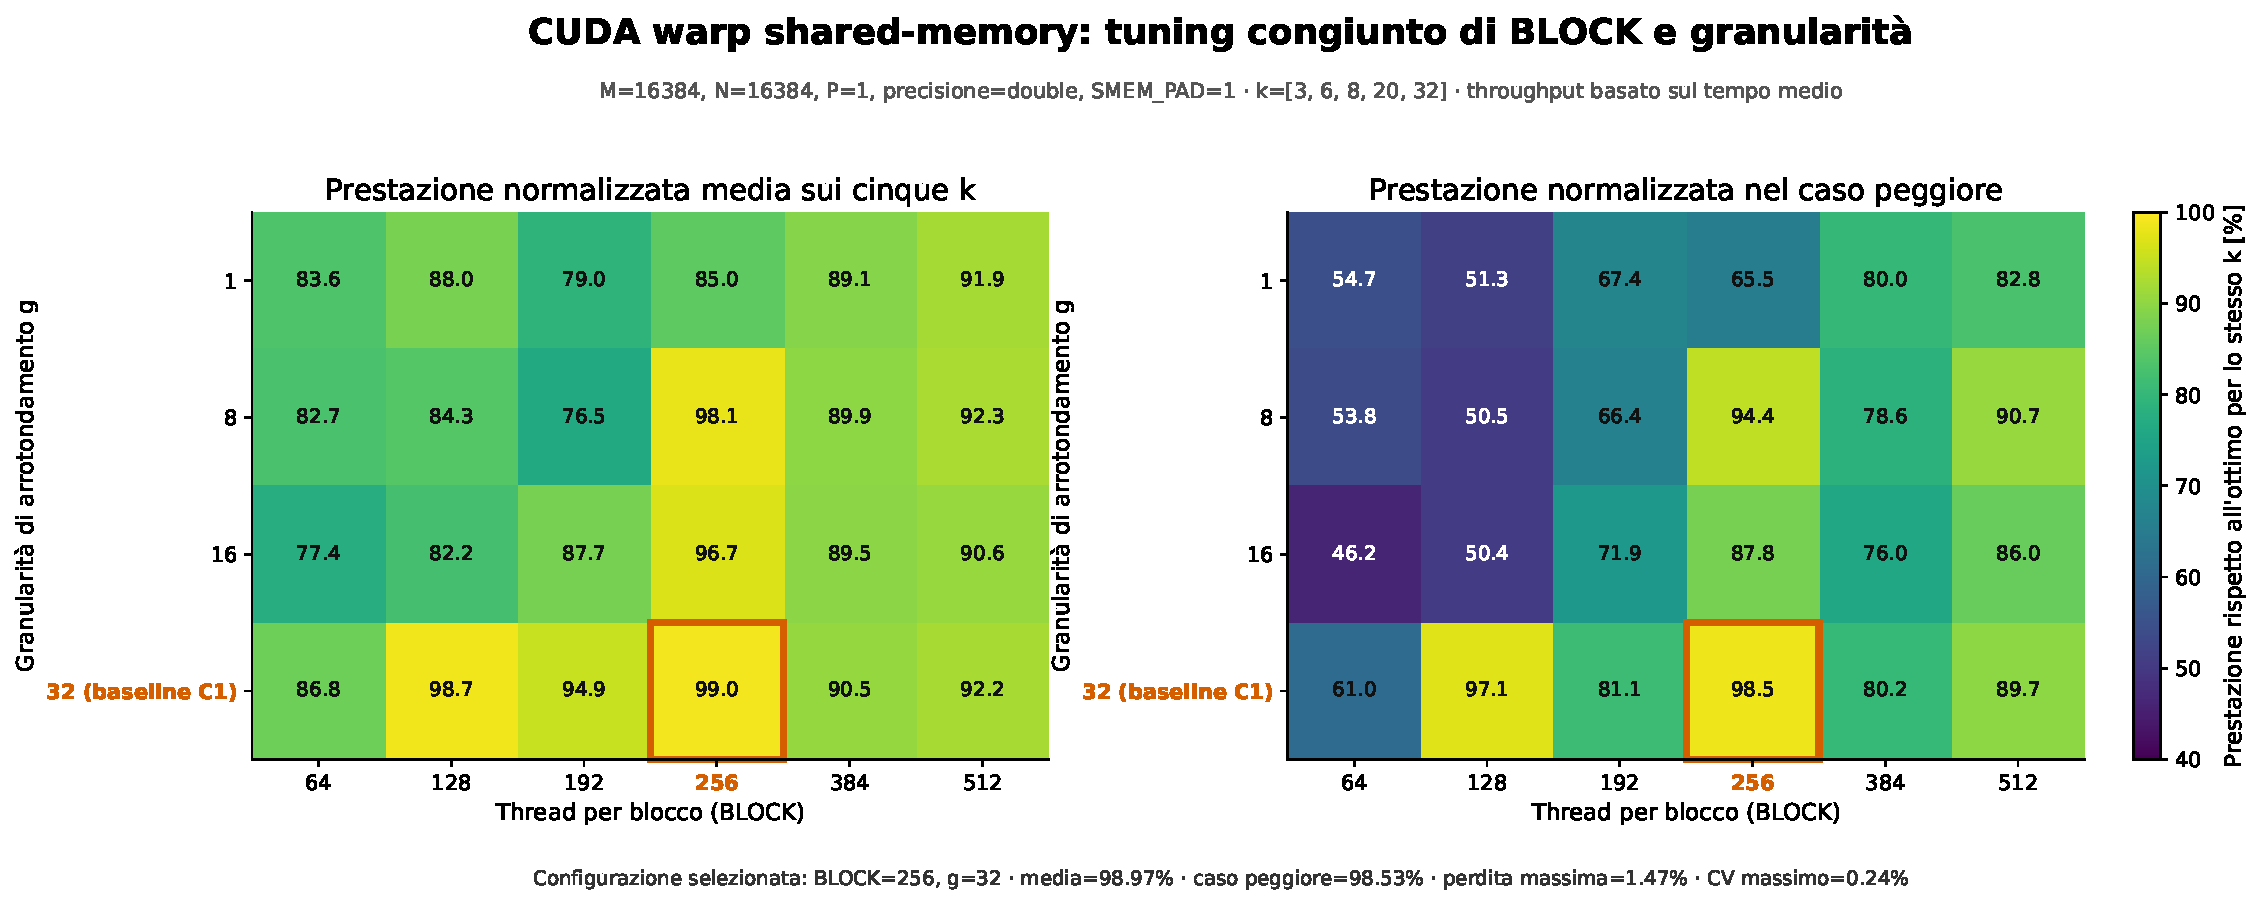
\includegraphics[width=\linewidth]{img/fase1/campagna_VAS_5_smem_granularity_tuning/campagna_VAS_5_joint_tuning_summary}
\caption{Campagna 1.4: tuning congiunto di \code{BLOCK} e granularità. A
sinistra la prestazione normalizzata media sui cinque $k$, a destra il caso
peggiore.}
\label{fig:ris-granularita}
\end{figure}

\begin{figure}[H]
\centering
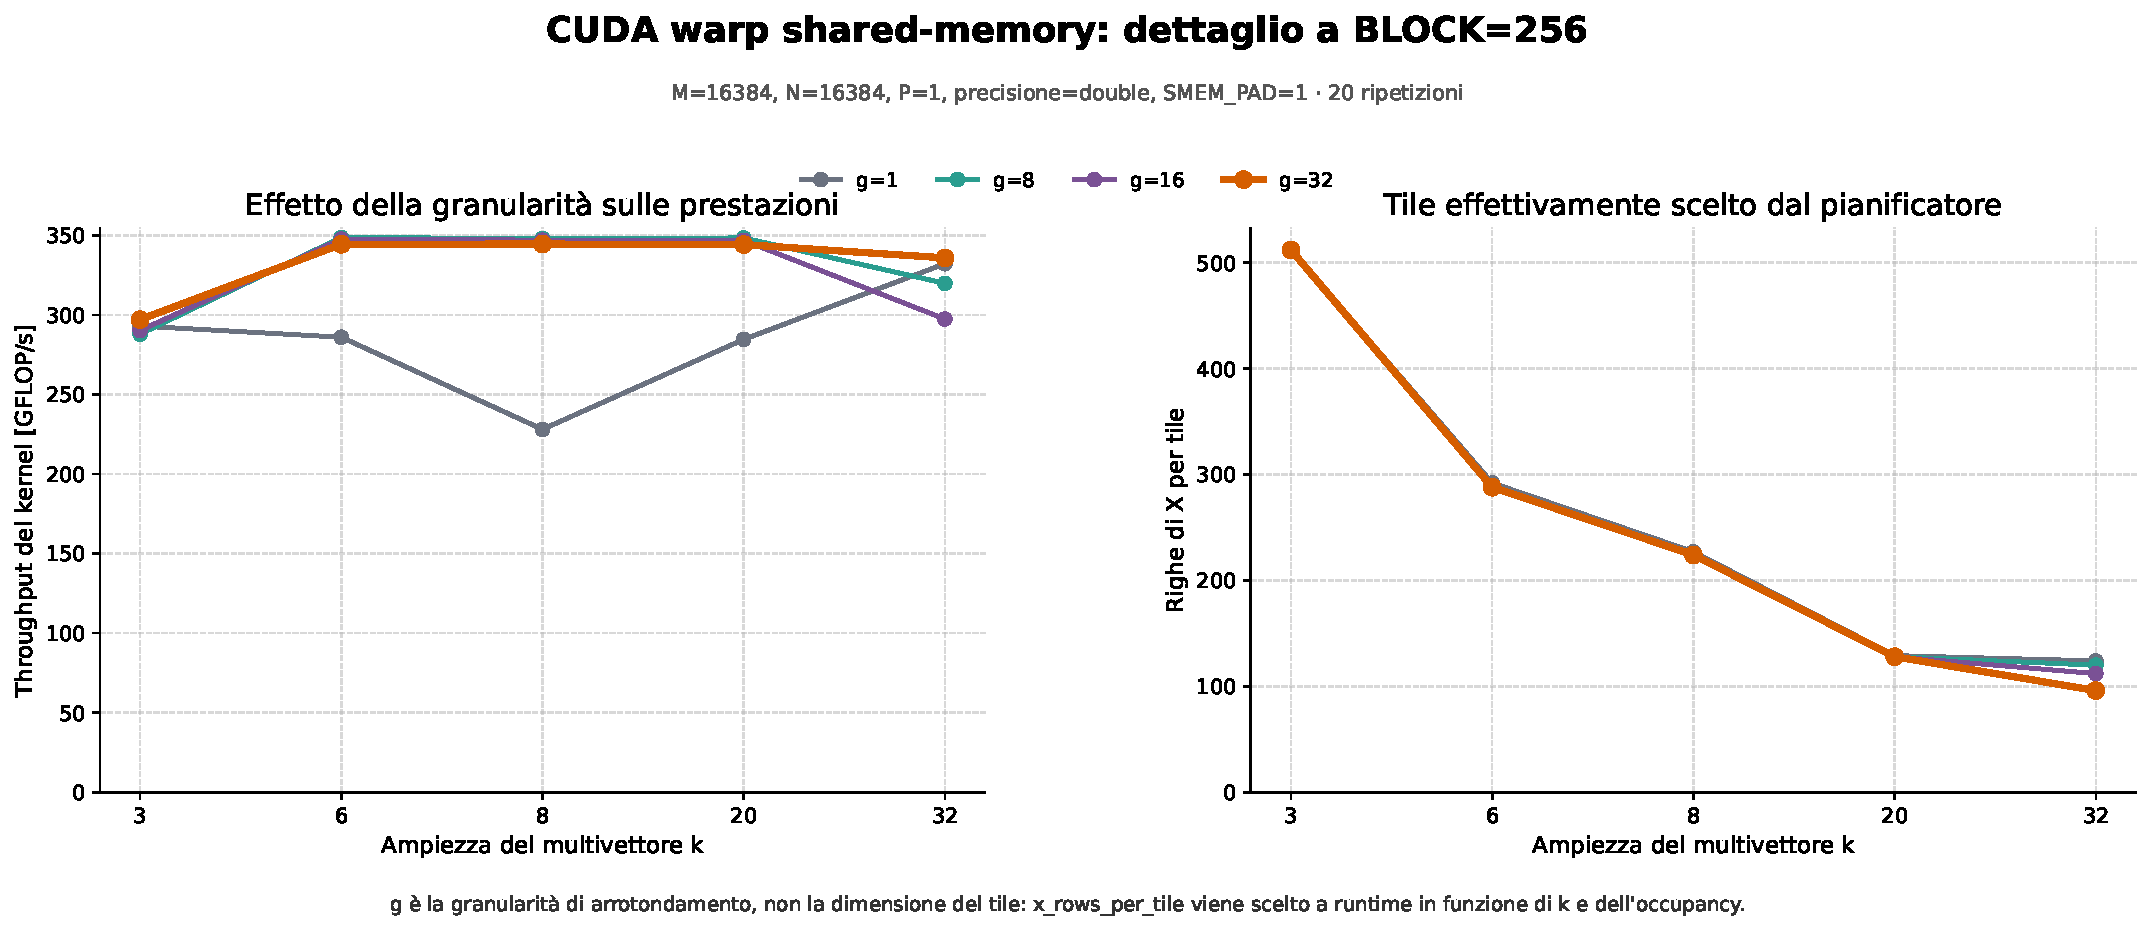
\includegraphics[width=\linewidth]{img/fase1/campagna_VAS_5_smem_granularity_tuning/campagna_VAS_5_block256_detail}
\caption{Campagna 1.4: dettaglio a \code{BLOCK}$=256$. A destra il piano di
tiling effettivamente scelto a runtime, che dipende da $k$ e non da $g$ se non
attraverso l'arrotondamento.}
\label{fig:ris-granularita-dettaglio}
\end{figure}

\subsubsection*{Lettura}

\textbf{Lo sweep congiunto conferma che \code{BLOCK} e granularità non possono
essere scelti indipendentemente.}

La configurazione preferibile cambia infatti al variare di $g$. Con
$g=1$ il valore medio più alto si ottiene a \code{BLOCK}=512, mentre per
$g=8$, $g=16$ e $g=32$ il miglior valore medio si trova a
\code{BLOCK}=256. Anche il comportamento nel caso peggiore cambia con la
coppia considerata.

La dimensione del blocco influenza il numero di warp che cooperano nello
stesso blocco e le risorse che determinano l'\emph{occupancy}, mentre la granularità
interviene successivamente sulla dimensione del tile scelta dal
pianificatore. I due parametri agiscono quindi sullo stesso kernel attraverso
meccanismi distinti, ma non indipendenti.

\textbf{Fra le granularità considerate, $g=32$ mostra il comportamento più
robusto.}

Essa fornisce la migliore prestazione media per cinque delle sei dimensioni
di blocco considerate, con l'unica eccezione di \code{BLOCK}=512, dove
$g=8$ e $g=32$ risultano sostanzialmente equivalenti. In particolare, la
coppia

\[
(\code{BLOCK},g)=(256,32)
\]

mantiene in media il $99{,}0\%$ della migliore prestazione ottenibile per
ciascun $k$ e non scende sotto il $98{,}5\%$ nel caso peggiore.

Il risultato è coerente con il ruolo di \code{TILE\_GRANULARITY} nel kernel.
Il ciclo di consumo della shared memory assegna alla lane $\ell$ le righe

\[
j=\ell,\;\ell+32,\;\ell+64,\ldots
\]

del tile. Quando il numero di righe è multiplo di 32, tutte le lane
completano lo stesso numero di passi. Una dimensione non multipla di 32 può
invece produrre un'ultima iterazione nella quale soltanto una parte delle
lane ha ancora una riga da elaborare.

Questo non implica tuttavia che una granularità pari a 32 sia
intrinsecamente ottimale. Arrotondare il tile a multipli più grandi può
lasciare inutilizzata una parte del budget di shared memory e aumentare il
numero complessivo di tile, e quindi delle sincronizzazioni. La campagna
misura proprio il bilancio fra questi due effetti.

\textbf{La granularità rifinisce un piano determinato principalmente dal
budget di shared memory.}

Come mostra \cref{fig:ris-granularita-dettaglio}, le diverse granularità non
producono piani radicalmente differenti. Il pianificatore determina prima
quante righe sono compatibili con il budget disponibile e con l'obiettivo di
occupancy, quindi arrotonda tale valore secondo $g$ e verifica nuovamente il
numero di blocchi residenti.

Per questo motivo \code{TILE\_GRANULARITY} non determina da sola la
dimensione del tile. Ne modifica piuttosto il valore finale attorno a una
dimensione già imposta dalle risorse disponibili. L'effetto prestazionale
può quindi essere ridotto quando i diversi arrotondamenti conducono a tile
simili, oppure diventare più evidente quando cambiano il numero di passi
necessari per attraversare $X$ e, di conseguenza, il numero di
sincronizzazioni eseguite dal blocco.

\subsection{Campagna 1.4 - Padding del tile in shared memory}
\label{sec:ris-pad}

\begin{table}[H]
\centering
\footnotesize
\caption{Campagna 1.4: effetto di \code{SMEM\_PAD} su
\kernelname{cuda\_warp\_smem}, \code{BLOCK}$=256$. \code{x\_rows\_per\_tile} è
il numero di righe di $X$ che il pianificatore fa entrare nel tile.}
\label{tab:ris-pad}
\begin{tabular}{@{}rrrrrr@{}}
\toprule
$k$ & \code{PAD}=0 & \code{PAD}=1 & guadagno & \code{x\_rows} & \code{x\_rows} \\
    & [GFLOPS] & [GFLOPS] & & \code{PAD}=0 & \code{PAD}=1 \\
\midrule
3  & 292,8 & 296,7 & $+1{,}3\%$  & 672 & 512 \\
6  & 315,8 & 351,8 & $+11{,}4\%$ & 320 & 288 \\
8  & 327,5 & 352,4 & $+7{,}6\%$  & 256 & 224 \\
20 & 353,9 & 352,2 & $-0{,}5\%$  & 128 & 128 \\
32 & 177,1 & 343,7 & $+94{,}1\%$ & 128 & 96 \\
\bottomrule
\end{tabular}
\end{table}

\begin{figure}[H]
\centering
\begin{tikzpicture}
\begin{axis}[
  scpa,
  width=0.82\linewidth,
  height=5.8cm,
  xlabel={$k$},
  ylabel={GFLOPS (kernel-only)},
  xmin=0,
  xmax=35,
  ymin=150,
  ymax=370,
  xtick={3,6,8,20,32},
  legend pos=south west
]
\addplot[blue!70!black,mark=*] coordinates {
  (3,292.840) (6,315.799) (8,327.543) (20,353.851) (32,177.113)
};
\addlegendentry{\code{SMEM\_PAD}=0}
\addplot[orange!80!black,mark=square*] coordinates {
  (3,296.715) (6,351.835) (8,352.396) (20,352.218) (32,343.740)
};
\addlegendentry{\code{SMEM\_PAD}=1}
\end{axis}
\end{tikzpicture}
\caption{Campagna 1.3: confronto fra tile senza padding e con una colonna di
padding. Il caso $k=32$ rende visibile la patologia che negli altri punti è
parzialmente nascosta dal resto del lavoro del kernel.}
\label{fig:ris-pad}
\end{figure}

\subsubsection*{Lettura}

\textbf{Il caso $k=32$ conferma il comportamento patologico previsto per la
mappatura sui bank.}

Senza padding, la distanza fra due righe consecutive del tile è pari a
$k=32$ elementi. In doppia precisione ciascun elemento occupa due parole da
32 bit, quindi lo spostamento fra gli indirizzi iniziali letti da lane
consecutive vale

\[
2\cdot32 = 64 \equiv 0 \pmod{32}.
\]

Gli accessi ricadono quindi periodicamente sugli stessi bank, producendo un
forte conflitto durante la lettura del tile dalla shared memory.

Con \code{SMEM\_PAD}=1 lo stride diventa invece $33$ elementi e lo
spostamento corrispondente vale

\[
2\cdot33 = 66 \equiv 2 \pmod{32},
\]

rompendo la periodicità del caso precedente. Il risultato sperimentale è
coerente con questa previsione: a $k=32$ il throughput passa da
$177{,}1$ a $343{,}7$ GFLOPS, con un incremento del $94{,}1\%$.

Il guadagno complessivo del kernel non deve però essere interpretato come
misura diretta della molteplicità del bank conflict. Il conflitto interessa
infatti soltanto la fase in cui $X$ viene letto dalla shared memory, mentre il
tempo totale comprende anche caricamento del tile, accessi ad $A$, operazioni
aritmetiche, riduzione e sincronizzazioni.

\textbf{Negli altri valori di $k$ l'effetto del padding è meno regolare.}

Il guadagno vale $11{,}4\%$ a $k=6$ e $7{,}6\%$ a $k=8$, mentre a
$k=20$ le due configurazioni differiscono soltanto dello $0{,}5\%$ a favore
della variante senza padding. A $k=3$ il vantaggio è invece limitato
all'$1{,}3\%$.

Questi risultati mostrano che la semplice regola modulare è utile per
individuare configurazioni chiaramente patologiche, come $k=32$, ma non
costituisce da sola un modello quantitativo delle prestazioni. Il tempo
complessivo dipende anche dalla dimensione effettiva del tile, dal numero di
blocchi residenti e dalla parte del kernel non coinvolta negli accessi alla
shared memory.

\textbf{Il padding migliora il caso peggiore al costo di una minore capacità
utile del tile.}

Aggiungere una colonna modifica la dimensione di ogni riga da $k$ a $k+1$
elementi. A parità di budget di shared memory possono quindi essere mantenute
meno righe di $X$ nello stesso tile. Ad esempio, il pianificatore passa da
672 a 512 righe per $k=3$ e da 128 a 96 per $k=32$.

Le righe che non entrano nel tile corrente non vengono escluse dal calcolo,
ma vengono elaborate nei tile successivi. Il costo potenziale del padding è
quindi una riduzione della quantità di $X$ trattata in ciascuna iterazione del
tiling e, in alcuni casi, un aumento del numero complessivo di tile e delle
relative sincronizzazioni.

Nonostante questo costo, il peggioramento massimo osservato con
\code{SMEM\_PAD}=1 è soltanto dello $0{,}5\%$, mentre nel caso patologico
$k=32$ il vantaggio è vicino a un fattore due. La scelta del padding è quindi
fortemente favorevole secondo il criterio di robustezza adottato nella
Fase~1.

\textbf{Esito della campagna.}

La configurazione selezionata è quindi:

\[
\code{SMEM\_PAD}=1.
\]

\textbf{Ripercussioni sul tuning congiunto.}

Combinando questo risultato con la scelta
\code{TILE_GRANULARITY}=32 della Campagna~1.3, la configurazione definitiva di
\kernelname{cuda\_warp\_smem} diventa

\[
(\code{BLOCK},\code{SMEM\_PAD},g)=(256,1,32).
\]


Nello sweep congiunto la coppia $(256,32)$ presenta una perdita massima
dell'$1{,}5\%$ rispetto alla migliore configurazione specifica per ciascun
$k$. La scelta soddisfa quindi il criterio di robustezza adottato nella
Fase~1 e definisce definitivamente il valore di
\code{BLOCK}.

\subsection{Esito della Fase 1 - Configurazioni consolidate}
\label{sec:ris-fase1-sintesi}

Le quattro campagne precedenti determinano le configurazioni utilizzate
nelle fasi successive. I valori selezionati sono raccolti in
\cref{tab:ris-fase1-sintesi}.

\begin{table}[H]
\centering
\footnotesize
\caption{Configurazione selezionata per ciascun backend CUDA.}
\label{tab:ris-fase1-sintesi}
\begin{tabular}{@{}llll@{}}
\toprule
\textbf{Backend} & \textbf{\code{BLOCK}} & \textbf{Layout di $X$} & \textbf{Altro} \\
\midrule
\kernelname{cuda\_naive}      & 128 & row    & - \\
\kernelname{cuda\_warp}       & 128 & column & - \\
\kernelname{cuda\_warp\_smem} & 256 & row    & \code{SMEM\_PAD}=1, $g=32$ \\
\kernelname{cublas}           & -   & row    & riferimento esterno \\
\bottomrule
\end{tabular}
\end{table}

Per \kernelname{cuda\_naive} e \kernelname{cuda\_warp} la dimensione del
blocco deriva dalla Campagna~1.1. Per \kernelname{cuda\_warp} la
Campagna~1.2 seleziona inoltre il layout column-major di $X$. Le
Campagne~1.3 e~1.4 completano invece la configurazione di
\kernelname{cuda\_warp\_smem}, selezionando rispettivamente il padding e la
coppia $(\code{BLOCK},\code{TILE\_GRANULARITY})$.

Da questo punto in avanti i parametri dei backend rimangono invariati.
Le fasi successive modificano quindi le caratteristiche del problema o
dell'aritmetica, senza introdurre un nuovo tuning.










\section{Fase 2 - Caratterizzazione dimensionale}
\label{sec:ris-fase2}

La Fase~1 ha fissato, per ciascun backend CUDA, una configurazione definitiva.
Tutte quelle misure sono però state prese su un unico problema,
$M=N=\num{16384}$. Resta quindi aperta una domanda: quei risultati valgono
solo per quella taglia, oppure descrivono un comportamento più generale?

La Fase~2 risponde variando le dimensioni del problema e separando due effetti
che nella pratica si presentano sempre insieme:

\begin{itemize}
  \item la \textbf{scala}, cioè quanto è grande il problema;
  \item la \textbf{forma}, cioè il rapporto fra il numero di righe $M$ e il
  numero di colonne $N$, a parità di lavoro complessivo.
\end{itemize}

Le due domande vengono affrontate una alla volta. Prima si tiene la matrice
quadrata e si fa crescere la taglia; poi si fissa la taglia e si cambia la
forma lasciando il lavoro quasi invariato.


\subsection{Disegno della campagna}
\label{sec:ris-fase2-disegno}

La campagna considera tre scale nominali

\[
S \in \{4096,\ 8192,\ \num{16384}\}
\]

e, per ciascuna scala, tre geometrie: il caso quadrato $M=N$, il caso
``largo'' $N=2M$ e il caso ``alto'' $M=3N$. I nove punti sono

\begin{center}
\footnotesize
\begin{tabular}{@{}lccc@{}}
\toprule
& $M=N$ & $N=2M$ & $M=3N$ \\
\midrule
$S=4096$  & $4096\times4096$   & $2880\times5760$   & $7104\times2368$ \\
$S=8192$  & $8192\times8192$   & $5760\times\num{11520}$  & $\num{14208}\times4736$ \\
$S=\num{16384}$ & $\num{16384}\times\num{16384}$ & $\num{11520}\times\num{23040}$ & $\num{28416}\times9472$ \\
\bottomrule
\end{tabular}
\end{center}

Le dimensioni rettangolari non sono scelte a caso: sono state costruite in modo
che il prodotto $MN$ resti quasi uguale a quello del caso quadrato della stessa
scala. Rispetto a $S^2$, la forma $N=2M$ ha l'$1{,}12\%$ di elementi in meno e
la forma $M=3N$ lo $0{,}27\%$ in più.

Questo dettaglio è ciò che rende interpretabile il confronto. Poiché il numero
di operazioni è
$2MNk$,
tenere $MN$ costante significa tenere costante il lavoro. Se due forme della
stessa scala danno throughput diversi, la differenza non può essere attribuita
al fatto che una delle due ``fa più conti'': è una reazione del kernel alla
geometria.

Tutte le misure sono in doppia precisione, con $P=1$, $5$ warm-up e $20$
repetition misurate, e usano per ogni backend i parametri selezionati nella
Fase~1 (\cref{sec:ris-fase1-sintesi}). La grandezza riportata è sempre
\code{gflops\_kernel}, cioè il throughput del solo kernel, al netto dei
trasferimenti H2D e D2H. Il prodotto completo dei fattori dà
$3$ scale $\times$ $3$ forme $\times$ $4$ backend $\times$ $5$ valori di $k$,
cioè $180$ configurazioni misurate.


\subsection{Effetto della scala}
\label{sec:ris-fase2-scala}

Per isolare la scala si guardano soltanto le configurazioni quadrate,
$M=N=S$,
facendo crescere $S$ di un fattore $2$ per volta, cioè facendo crescere il
lavoro di un fattore $4$ per volta.

\begin{table}[H]
\centering
\footnotesize
\caption{Fase~2: \code{gflops\_kernel} dei quattro backend sul caso quadrato
$M=N=S$, per tutti i valori di $k$ misurati.}
\label{tab:ris-fase2-scala-completa}
\begin{tabular}{@{}llrrrrr@{}}
\toprule
\textbf{Scala} & \textbf{Backend}
& $k=3$ & $k=6$ & $k=8$ & $k=20$ & $k=32$ \\
\midrule

\multirow{4}{*}{$S=4096$}
& \kernelname{cuda\_naive} & 162,3 & 252,0 & 253,2 & 277,2 & 287,7 \\
& \kernelname{cuda\_warp} & 269,6 & 275,7 & 277,4 & 279,8 & 281,5 \\
& \kernelname{cuda\_warp\_smem} & 253,5 & 265,8 & 267,5 & 273,5 & 274,5 \\
& \kernelname{cublas} & 16,5 & 34,6 & 46,1 & 115,2 & 184,3 \\

\midrule

\multirow{4}{*}{$S=8192$}
& \kernelname{cuda\_naive} & 187,3 & 309,7 & 342,5 & 348,7 & 354,5 \\
& \kernelname{cuda\_warp} & 297,5 & 348,4 & 347,8 & 347,5 & 354,1 \\
& \kernelname{cuda\_warp\_smem} & 291,5 & 338,3 & 337,6 & 338,6 & 330,7 \\
& \kernelname{cublas} & 15,4 & 30,8 & 41,1 & 102,7 & 164,0 \\

\midrule

\multirow{4}{*}{$S=\num{16384}$}
& \kernelname{cuda\_naive} & 151,5 & 307,1 & 342,0 & 345,5 & 349,7 \\
& \kernelname{cuda\_warp} & 302,0 & 354,3 & 353,2 & 354,6 & 354,9 \\
& \kernelname{cuda\_warp\_smem} & 296,8 & 349,8 & 349,6 & 349,5 & 341,0 \\
& \kernelname{cublas} & 15,3 & 30,7 & 40,8 & 102,0 & 163,2 \\

\bottomrule
\end{tabular}
\end{table}

Una prima lettura della \cref{tab:ris-fase2-scala-completa} mostra due
comportamenti opposti. I tre kernel scritti nel progetto migliorano al
crescere della taglia; \kernelname{cublas} peggiora. Inoltre, per i kernel
custom quasi tutto il guadagno si concentra nel primo raddoppio, da $S=4096$ a
$S=8192$: il passaggio successivo aggiunge poco.

\subsubsection{\kernelname{cuda\_warp}}

Il caso più netto è \kernelname{cuda\_warp}. Alla scala più piccola il
throughput è praticamente insensibile a $k$: resta fra $269{,}6$ e
$281{,}5$ GFLOPS su tutto l'intervallo, cioè si muove di poco più di
$10$ GFLOPS mentre il lavoro cresce di dieci volte.

Alle due scale maggiori il comportamento cambia forma. Il valore a $k=3$ resta
isolato in basso ($297{,}5$ e $302{,}0$ GFLOPS), mentre da $k=6$ in poi il
kernel si appiattisce su un plateau: $347{,}5$–$354{,}1$ GFLOPS a $S=8192$ e
$353{,}2$–$354{,}9$ GFLOPS a $S=\num{16384}$.

Il confronto fra la prima e l'ultima scala si riassume in due numeri:

\begin{itemize}
  \item per $k\ge6$ il guadagno sta fra $1{,}26$ e $1{,}29\times$;
  \item a $k=3$ è solo di circa $1{,}12\times$.
\end{itemize}

Il punto importante non è però l'entità del guadagno, ma il fatto che a
$S=4096$ il plateau \emph{non viene mai raggiunto}, per nessun valore di $k$.
A $S=4096$ e $k=32$ il kernel fa $281{,}5$ GFLOPS, contro i $354{,}9$ dello
stesso kernel e dello stesso $k$ a $S=\num{16384}$: la differenza non dipende
dalla larghezza del multivettore, ma dalla taglia del problema.

Una taglia più piccola significa meno lavoro per singola invocazione e quindi
meno righe di $Y$ da produrre, cioè meno warp indipendenti disponibili. Le sole
misure temporali non permettono però di attribuire il deficit a un meccanismo
preciso (occupancy, latenza, comportamento delle cache o numero di blocchi
residenti). L'affermazione che i dati sostengono direttamente è più semplice e
più utile: \kernelname{cuda\_warp} raggiunge il proprio regime di plateau
soltanto quando il problema è abbastanza grande, e $S=4096$ è al di sotto di
quella soglia.

\begin{figure}[H]
\centering
\begin{tikzpicture}
\begin{axis}[
  scpa,
  xlabel={$k$},
  ylabel={GFLOPS (kernel-only)},
  xmin=0,
  xmax=35,
  ymin=240,
  ymax=410,
  xtick={3,6,8,20,32},
  legend pos=north west,
  width=0.8\linewidth,
  height=6cm
]

\addplot[black, dashed, thick, forget plot, samples=2, domain=0:35]{350};

\addplot[blue!70!black, mark=*] coordinates {
  (3,302.0) (6,354.3) (8,353.2) (20,354.6) (32,354.9)
};
\addlegendentry{$S=16384$}

\addplot[teal!70!black, mark=triangle*] coordinates {
  (3,297.5) (6,348.4) (8,347.8) (20,347.5) (32,354.1)
};
\addlegendentry{$S=8192$}

\addplot[orange!80!black, mark=square*] coordinates {
  (3,269.6) (6,275.7) (8,277.4) (20,279.8) (32,281.5)
};
\addlegendentry{$S=4096$}

\end{axis}
\end{tikzpicture}

\caption{Fase~2: \kernelname{cuda\_warp} sul caso quadrato alle tre scale,
dai valori della \cref{tab:ris-fase2-scala-completa}. La linea tratteggiata
indica il tetto FP64 nominale di \SI{350}{\giga\flop\per\second} utilizzato
nel modello.}
\label{fig:ris-fase2-scala}
\end{figure}

La figura rende visibile la differenza qualitativa: a $S=4096$ la curva è
piatta e lontana dal tetto, alle due scale maggiori sale subito e poi si
appoggia sul tetto.

\subsubsection{\kernelname{cuda\_warp\_smem}}

La variante con shared memory segue lo stesso andamento generale, ma in modo
più graduale e senza mai superare \kernelname{cuda\_warp} sul caso quadrato.

A differenza degli altri due kernel custom, qui la crescita con la scala è
monotona per ogni $k$: a $k=3$ i tre valori sono $253{,}5$, $291{,}5$ e
$296{,}8$ GFLOPS; a $k=32$ sono $274{,}5$, $330{,}7$ e $341{,}0$ GFLOPS. Il
throughput continua quindi ad aumentare anche nel passaggio da $S=8192$ a
$S=\num{16384}$, dove \kernelname{cuda\_warp} si era già fermato.

Lo scarto rispetto a \kernelname{cuda\_warp} resta comunque sempre a favore di
quest'ultimo. Alle due scale maggiori è piccolo, entro il $3\%$ per $k\le20$;
a $S=4096$ è un po' più ampio e vale il $6{,}3\%$ a $k=3$ ($269{,}6$ contro
$253{,}5$). Fa eccezione $k=32$, dove il divario si allarga anche sui problemi
grandi ($330{,}7$ contro $354{,}1$ a $S=8192$ e $341{,}0$ contro $354{,}9$ a
$S=\num{16384}$).

Si nota anche, alle due scale maggiori, un piccolo calo passando da $k=20$ a
$k=32$ ($338{,}6 \rightarrow 330{,}7$ e $349{,}5 \rightarrow 341{,}0$), che
sulle altre due varianti non compare. È l'unico punto della campagna in cui
lo staging esplicito di $X$ in shared memory sembra costare più di quanto
rende in FP64.

\subsubsection{\kernelname{cuda\_naive}}

Il kernel di riferimento interno ha un andamento meno regolare, e il motivo è
concentrato tutto a $k=3$.

Per $k\ge8$ \kernelname{cuda\_naive} cresce con la scala e arriva dove
arrivano gli altri: $342{,}0$–$349{,}7$ GFLOPS a $S=\num{16384}$, cioè
sostanzialmente il valore di \kernelname{cuda\_warp}. A $k=3$, invece, la
successione è

\[
162{,}3 \rightarrow 187{,}3 \rightarrow 151{,}5 \quad\text{GFLOPS},
\]

cioè non monotona: il valore migliore si osserva alla scala intermedia e quello
peggiore alla scala massima.

Il confronto fra i due kernel a $k=3$ è quindi il risultato più stabile della
tabella, e non si attenua crescendo: \kernelname{cuda\_warp} vale
$1{,}66\times$ a $S=4096$ e arriva a $1{,}99\times$ a $S=\num{16384}$. Il
vantaggio della mappatura a warp non è un throughput di picco più alto, ma il
fatto di raggiungerlo già con multivettori stretti.

\subsubsection{\kernelname{cublas}}

Il riferimento esterno si comporta in modo qualitativamente diverso da tutti i
kernel custom, e la tabella lo mostra senza bisogno di altre misure.

Si prenda la riga $S=\num{16384}$ e si parta da $k=3$, dove il valore è
$15{,}3$ GFLOPS. Moltiplicando per $k/3$ si ottiene $30{,}6$, $40{,}8$,
$102{,}0$ e $163{,}2$, contro i $30{,}7$, $40{,}8$, $102{,}0$ e $163{,}2$
effettivamente misurati. Il throughput è quindi \emph{proporzionale} a $k$, e
poiché

\[
\text{GFLOPS} = \frac{2MNk}{t_{\text{kernel}}},
\]

questo equivale a dire che $t_{\text{kernel}}$ non dipende da $k$. La stessa
verifica riesce a $S=8192$ e, da $k=6$ in poi, anche a $S=4096$.

Il costo della chiamata è dunque determinato dallo streaming di $A$, non dal
lavoro effettivamente richiesto: con $k\le32$ una GEMM general-purpose paga
quasi lo stesso tempo che pagherebbe per un multivettore molto più largo.

Sulla scala, cuBLAS perde invece throughput: a ogni $k$ il valore a $S=8192$
è circa l'$89\%$ di quello a $S=4096$, e a $S=\num{16384}$ resta lì. Il
divario rispetto a \kernelname{cuda\_warp} sul problema più grande va da
$19{,}7\times$ a $k=3$ a $2{,}2\times$ a $k=32$: si riduce al crescere di $k$,
come previsto, ma non si annulla nell'intervallo richiesto dalla traccia.


\subsection{Effetto della forma}
\label{sec:ris-fase2-forma}

La seconda domanda riguarda la geometria. Per ogni scala si confrontano le tre
forme $M=N$, $N=2M$ e $M=3N$, che come detto hanno lo stesso $MN$ entro
l'$1{,}2\%$.

Il confronto va letto così: a parità di scala e di $k$, il numero di
operazioni è lo stesso in tutte e tre le righe di una tabella, quindi ogni
differenza verticale è sensibilità alla forma. Un modo compatto per
riassumere ciascun blocco è lo \emph{scarto} fra la forma migliore e la
peggiore, espresso in percentuale della peggiore.

\subsubsection{\kernelname{cuda\_warp}}

\begin{table}[H]
\centering
\footnotesize
\caption{Fase~2: \code{gflops\_kernel} di \kernelname{cuda\_warp} sulle tre
forme e sulle tre scale.}
\label{tab:ris-fase2-warp}
\begin{tabular}{@{}llrrrrr@{}}
\toprule
\textbf{Scala} & \textbf{Forma}
& $k=3$ & $k=6$ & $k=8$ & $k=20$ & $k=32$ \\
\midrule

\multirow{3}{*}{$S=4096$}
& $M=N$  & 269,6 & 275,7 & 277,4 & 279,8 & 281,5 \\
& $N=2M$ & 280,8 & 308,9 & 310,4 & 289,0 & 292,0 \\
& $M=3N$ & 285,7 & 330,0 & 330,5 & 278,0 & 281,4 \\

\midrule

\multirow{3}{*}{$S=8192$}
& $M=N$  & 297,5 & 348,4 & 347,8 & 347,5 & 354,1 \\
& $N=2M$ & 296,6 & 353,5 & 351,5 & 354,7 & 357,5 \\
& $M=3N$ & 297,8 & 343,1 & 342,7 & 345,9 & 347,6 \\

\midrule

\multirow{3}{*}{$S=\num{16384}$}
& $M=N$  & 302,0 & 354,3 & 353,2 & 354,6 & 354,9 \\
& $N=2M$ & 300,0 & 356,0 & 355,8 & 357,4 & 356,7 \\
& $M=3N$ & 301,7 & 349,6 & 349,8 & 351,9 & 352,4 \\

\bottomrule
\end{tabular}
\end{table}

Alla scala più piccola la forma conta molto. A $S=4096$ e $k=6$ il throughput
passa da $275{,}7$ GFLOPS nel caso quadrato a $308{,}9$ per $N=2M$ e
$330{,}0$ per $M=3N$; a $k=8$ l'andamento è quasi identico
($277{,}4 \rightarrow 310{,}4 \rightarrow 330{,}5$). In entrambi i casi lo
scarto fra la forma migliore e la peggiore è vicino al $20\%$.

Non esiste però una forma sempre vincente, nemmeno a scala fissa. Sulla stessa
riga di scala, a $k=20$ la migliore è $N=2M$ ($289{,}0$ contro $279{,}8$ e
$278{,}0$) e a $k=32$ vale lo stesso ($292{,}0$ contro $281{,}5$ e $281{,}4$).
La forma $M=3N$, che era la migliore ai $k$ stretti, diventa la peggiore ai
$k$ larghi. L'effetto della geometria dipende quindi anche da $k$.

Crescendo di scala la dispersione crolla. A $S=8192$ lo scarto massimo su
tutti i $k$ è del $3{,}1\%$, a $S=\num{16384}$ dell'$1{,}8\%$: a $k=6$, per
esempio, i tre valori sono $354{,}3$, $356{,}0$ e $349{,}6$ GFLOPS.

Questo comportamento si lega alla struttura del kernel. \kernelname{cuda\_warp}
assegna un warp a ogni riga di $Y$, quindi cambiare il rapporto $M{:}N$ a
prodotto costante modifica due cose insieme: quante righe indipendenti
esistono, e quanto è lunga la riduzione lungo $N$ che ciascun warp deve
percorrere. Nel caso $M=3N$ ci sono più righe ma riduzioni più corte; nel caso
$N=2M$ avviene il contrario.

La campagna non permette di separare quantitativamente i due effetti, e il
vantaggio di $M=3N$ a $S=4096$ non va quindi letto come prova che ``più righe
è meglio''. Il risultato solido è un altro: quando il problema è abbastanza
grande da fornire comunque parallelismo in abbondanza, la forma smette
praticamente di contare.

\subsubsection{\kernelname{cuda\_naive}}

\begin{table}[H]
\centering
\footnotesize
\caption{Fase~2: \code{gflops\_kernel} di \kernelname{cuda\_naive} sulle tre
forme e sulle tre scale.}
\label{tab:ris-fase2-naive}
\begin{tabular}{@{}llrrrrr@{}}
\toprule
\textbf{Scala} & \textbf{Forma}
& $k=3$ & $k=6$ & $k=8$ & $k=20$ & $k=32$ \\
\midrule

\multirow{3}{*}{$S=4096$}
& $M=N$  & 162,3 & 252,0 & 253,2 & 277,2 & 287,7 \\
& $N=2M$ & 149,9 & 274,2 & 329,1 & 275,5 & 300,7 \\
& $M=3N$ & 165,9 & 297,7 & 324,5 & 283,5 & 295,8 \\

\midrule

\multirow{3}{*}{$S=8192$}
& $M=N$  & 187,3 & 309,7 & 342,5 & 348,7 & 354,5 \\
& $N=2M$ & 160,3 & 284,8 & 326,0 & 345,6 & 356,5 \\
& $M=3N$ & 140,1 & 296,0 & 341,4 & 346,8 & 354,4 \\

\midrule

\multirow{3}{*}{$S=\num{16384}$}
& $M=N$  & 151,5 & 307,1 & 342,0 & 345,5 & 349,7 \\
& $N=2M$ & 134,0 & 277,4 & 349,9 & 342,0 & 347,6 \\
& $M=3N$ & 132,6 & 289,2 & 348,2 & 342,9 & 346,1 \\

\bottomrule
\end{tabular}
\end{table}

\kernelname{cuda\_naive} è il backend più sensibile alla forma, e soprattutto
è l'unico in cui la sensibilità \emph{non} sparisce crescendo di scala: cambia
solo il valore di $k$ in cui si manifesta.

A $S=4096$ il massimo scarto è del $30{,}0\%$ ed è a $k=8$ ($253{,}2$ nel caso
quadrato contro $329{,}1$ per $N=2M$): le forme rettangolari sono molto
migliori.

A $S=8192$ e $S=\num{16384}$ il segno si rovescia e il fenomeno si sposta a
$k=3$. Alla scala intermedia lo scarto è del $33{,}7\%$, il più grande
dell'intera campagna ($187{,}3$ per il quadrato contro $140{,}1$ per $M=3N$);
alla scala massima è ancora del $14{,}2\%$ ($151{,}5$ contro $132{,}6$).
Adesso è il caso quadrato a essere nettamente il migliore.

Per $k\ge20$, invece, le tre forme si avvicinano molto: lo scarto è del
$4{,}5\%$ a $S=4096$ e scende sotto l'$1\%$ alle due scale maggiori.

La lettura complessiva è coerente con quanto visto sulla scala: il punto
debole di \kernelname{cuda\_naive} sono i multivettori stretti, e proprio lì il
kernel resta esposto alla geometria del problema anche quando il problema è
grande.

\subsubsection{\kernelname{cuda\_warp\_smem}}

\begin{table}[H]
\centering
\footnotesize
\caption{Fase~2: \code{gflops\_kernel} di \kernelname{cuda\_warp\_smem} sulle
tre forme e sulle tre scale.}
\label{tab:ris-fase2-smem}
\begin{tabular}{@{}llrrrrr@{}}
\toprule
\textbf{Scala} & \textbf{Forma}
& $k=3$ & $k=6$ & $k=8$ & $k=20$ & $k=32$ \\
\midrule

\multirow{3}{*}{$S=4096$}
& $M=N$  & 253,5 & 265,8 & 267,5 & 273,5 & 274,5 \\
& $N=2M$ & 272,5 & 316,9 & 318,6 & 268,5 & 262,0 \\
& $M=3N$ & 282,3 & 312,3 & 319,2 & 268,5 & 263,0 \\

\midrule

\multirow{3}{*}{$S=8192$}
& $M=N$  & 291,5 & 338,3 & 337,6 & 338,6 & 330,7 \\
& $N=2M$ & 291,4 & 347,9 & 348,3 & 349,6 & 342,4 \\
& $M=3N$ & 293,6 & 338,0 & 338,7 & 341,5 & 333,8 \\

\midrule

\multirow{3}{*}{$S=\num{16384}$}
& $M=N$  & 296,8 & 349,8 & 349,6 & 349,5 & 341,0 \\
& $N=2M$ & 289,7 & 349,7 & 349,6 & 350,3 & 341,6 \\
& $M=3N$ & 295,8 & 346,9 & 345,8 & 347,3 & 338,8 \\

\bottomrule
\end{tabular}
\end{table}

La variante con shared memory riproduce la convergenza già vista per
\kernelname{cuda\_warp}: scarto massimo del $19{,}3\%$ a $S=4096$, del
$3{,}5\%$ a $S=8192$ e del $2{,}4\%$ a $S=\num{16384}$.

Alla scala piccola, però, l'effetto cambia segno con $k$ in modo molto
marcato. A $k=6$ e $k=8$ le forme rettangolari vincono nettamente
($267{,}5 \rightarrow 318{,}6$ e $319{,}2$ a $k=8$), mentre a $k=20$ e $k=32$
perdono e il caso quadrato diventa il migliore ($274{,}5$ contro $262{,}0$ e
$263{,}0$ a $k=32$).

Alla scala intermedia emerge invece una regolarità pulita: per $k\ge6$ la
forma $N=2M$ è la migliore a tutti i valori di $k$, con un vantaggio di circa
il $3\%$ (a $k=3$ le tre forme sono già indistinguibili, entro lo $0{,}7\%$). Alla scala massima anche questo vantaggio si assottiglia e le tre
forme diventano intercambiabili.

Va sottolineato un punto che riguarda l'interpretazione. La configurazione del
backend resta identica lungo tutta la campagna: a parità di $k$, il numero di
blocchi residenti per SM e il numero di righe di $X$ caricate per tile non
cambiano al variare del rapporto $M{:}N$. Le differenze osservate fra le forme
non sono quindi riconducibili a una diversa scelta del piano di tiling.

\subsubsection{\kernelname{cublas}}

\begin{table}[H]
\centering
\footnotesize
\caption{Fase~2: \code{gflops\_kernel} di \kernelname{cublas} sulle tre
forme e sulle tre scale.}
\label{tab:ris-fase2-cublas}
\begin{tabular}{@{}llrrrrr@{}}
\toprule
\textbf{Scala} & \textbf{Forma}
& $k=3$ & $k=6$ & $k=8$ & $k=20$ & $k=32$ \\
\midrule

\multirow{3}{*}{$S=4096$}
& $M=N$  & 16,5 & 34,6 & 46,1 & 115,2 & 184,3 \\
& $N=2M$ & 13,6 & 32,5 & 43,4 & 108,2 & 173,4 \\
& $M=3N$ & 16,0 & 32,0 & 42,7 & 106,6 & 170,8 \\

\midrule

\multirow{3}{*}{$S=8192$}
& $M=N$  & 15,4 & 30,8 & 41,1 & 102,7 & 164,0 \\
& $N=2M$ & 16,3 & 32,5 & 43,4 & 108,2 & 173,5 \\
& $M=3N$ & 15,9 & 31,9 & 42,5 & 106,1 & 169,6 \\

\midrule

\multirow{3}{*}{$S=\num{16384}$}
& $M=N$  & 15,3 & 30,7 & 40,8 & 102,0 & 163,2 \\
& $N=2M$ & 16,0 & 32,1 & 42,8 & 106,9 & 170,9 \\
& $M=3N$ & 15,8 & 31,6 & 42,1 & 105,3 & 168,5 \\

\bottomrule
\end{tabular}
\end{table}

cuBLAS è l'unico backend in cui la sensibilità alla forma \emph{non} si riduce
crescendo di scala. Lo scarto resta intorno all'$8\%$ a $S=4096$ (per $k\ge6$),
al $5{,}7\%$ a $S=8192$ e al $4{,}9\%$ a $S=\num{16384}$.

Cambia però quale forma vince. A $S=4096$ il caso quadrato è il migliore a
tutti i $k$; alle due scale maggiori diventa il \emph{peggiore}, e la forma
$N=2M$ passa davanti ($170{,}9$ contro $163{,}2$ GFLOPS a $k=32$,
$S=\num{16384}$). Vale la pena notare che $N=2M$ è anche la forma con
l'$1{,}12\%$ di elementi in meno: il vantaggio osservato è quattro volte più
grande di quella differenza, quindi non è un artefatto del disegno.

Una parte della spiegazione è nel modo in cui il backend chiama la libreria. Il
prodotto row-major viene realizzato reinterpretando i buffer secondo la
convenzione column-major, e per $P=1$ la GEMM riceve dimensioni

\[
m_{\mathrm{GEMM}}=k,
\qquad
n_{\mathrm{GEMM}}=M,
\qquad
K_{\mathrm{GEMM}}=N.
\]

Cambiare il rapporto $M{:}N$ cambia quindi direttamente la geometria vista
dalla routine. I soli tempi non dicono però quale kernel interno o quale
tiling venga selezionato: una spiegazione microarchitetturale richiederebbe
una profilazione dedicata.

\subsubsection{Confronto fra i backend}

Mettendo insieme le quattro tabelle, la robustezza alla forma si riassume nello
scarto massimo osservato su tutti i $k$ di una stessa scala:

\begin{center}
\footnotesize
\begin{tabular}{@{}lrrr@{}}
\toprule
\textbf{Backend} & $S=4096$ & $S=8192$ & $S=\num{16384}$ \\
\midrule
\kernelname{cuda\_naive}      & $30{,}0\%$ & $33{,}7\%$ & $14{,}2\%$ \\
\kernelname{cuda\_warp}       & $19{,}7\%$ & $3{,}1\%$  & $1{,}8\%$ \\
\kernelname{cuda\_warp\_smem} & $19{,}3\%$ & $3{,}5\%$  & $2{,}4\%$ \\
\kernelname{cublas}           & $21{,}4\%$ & $5{,}7\%$  & $4{,}9\%$ \\
\bottomrule
\end{tabular}
\end{center}

I valori sono calcolati dalle tabelle precedenti come
$(\max-\min)/\min$ fra le tre forme, prendendo poi il caso peggiore sui cinque
$k$.

Alla scala più piccola tutti e quattro i backend sono sensibili alla geometria
in misura confrontabile, fra il $19\%$ e il $30\%$. È crescendo che i
comportamenti si separano: i due kernel a mappatura warp diventano
praticamente indifferenti alla forma, cuBLAS si stabilizza intorno al $5\%$ e
\kernelname{cuda\_naive} resta esposto per via del solo $k=3$.


\subsection{Sintesi della Fase 2}
\label{sec:ris-fase2-sintesi}

La Fase~2 porta tre conclusioni.

\paragraph{La scala conta, e conta una volta sola.}
Per i kernel custom il salto prestazionale avviene fra $S=4096$ e $S=8192$;
oltre, il guadagno è marginale. \kernelname{cuda\_warp} guadagna fra
$1{,}26$ e $1{,}29\times$ da $S=4096$ a $S=\num{16384}$ per $k\ge6$, ma quasi
tutto nel primo raddoppio. Il problema a $S=4096$ appartiene a un regime diverso: il
plateau non viene raggiunto per nessun $k$.

\paragraph{La forma conta soprattutto quando la scala è insufficiente.}
Le differenze vicine al $20\%$ osservate a $S=4096$ si riducono sotto il
$2\%$ per \kernelname{cuda\_warp} a $S=\num{16384}$. Non si tratta però di una
regola valida per tutti i backend: \kernelname{cuda\_naive} conserva un
$14{,}2\%$ di scarto a $k=3$ anche alla scala massima, e cuBLAS resta intorno
al $5\%$ a ogni scala. Scala, forma e larghezza del multivettore vanno quindi
considerate insieme, non come fattori indipendenti.

\paragraph{Il comportamento di cuBLAS è strutturalmente diverso.}
Il throughput proporzionale a $k$ mostra che il tempo di kernel della libreria
non dipende dal lavoro richiesto: per $k\le32$ una GEMM general-purpose non
ammortizza il proprio percorso. Questo, e non un difetto di ottimizzazione,
è ciò che i kernel custom sfruttano.

\medskip

Su questa base la Fase~3 mantiene il problema

\[
M=N=\num{16384}.
\]

La scelta non implica che la geometria quadrata massima sia ottimale per ogni
backend. Fornisce però un punto in cui \kernelname{cuda\_warp} è nel proprio
plateau (circa $355$ GFLOPS per $k\ge6$, cioè poco oltre il tetto FP64
nominale di \SI{350}{\giga\flop\per\second}) ed è al tempo stesso il più
insensibile alla forma. Fissare quella geometria permette alla Fase~3 di
isolare l'effetto della precisione numerica senza cambiare
contemporaneamente dimensione e forma del problema. Nella Fase~4 la scala
torna invece a essere un fattore sperimentale, per osservare come la
composizione MPI + CUDA dipenda dalla dimensione del problema globale.
dipenda anche dalla dimensione del problema globale.


\section{Fase 3 - Effetto della precisione numerica}
\label{sec:ris-fase3}
\label{sec:c7}

Il riferimento FP64 è il punto $S = 16384$, $M = N$ della Fase 2. Le misure
FP32 sono nuove, sulle stesse configurazioni e con lo stesso protocollo.

\begin{table}[H]
\centering
\footnotesize
\caption{Fase 3: \code{gflops\_kernel} nelle due precisioni e speedup
$S_{32/64}$ della \cref{eq:speedup-precisione}, $M = N = \num{16384}$, $P = 1$.}
\label{tab:ris-fase3}
\begin{tabular}{@{}lrrrrr@{}}
\toprule
\textbf{Backend} & $k=3$ & $k=6$ & $k=8$ & $k=20$ & $k=32$ \\
\midrule
\multicolumn{6}{@{}l}{\itshape GFLOPS in FP32} \\
\kernelname{cuda\_naive}      & 198,3 & 386,8  & 522,0  & 791,6  & 1107,4 \\
\kernelname{cuda\_warp}       & 604,4 & 1169,8 & 1414,3 & 1489,3 & \textbf{1945,9} \\
\kernelname{cuda\_warp\_smem} & 601,2 & 1164,7 & 1457,2 & \textbf{1726,9} & 1473,0 \\
\kernelname{cublas}           & 426,7 & 861,1  & 1141,0 & 2962,3 & 4791,9 \\
\midrule
\multicolumn{6}{@{}l}{\itshape GFLOPS in FP64 (riferimento, Fase 2)} \\
\kernelname{cuda\_naive}      & 151,5 & 307,1 & 342,0 & 345,5 & 349,7 \\
\kernelname{cuda\_warp}       & 302,0 & 354,3 & 353,2 & 354,6 & 354,9 \\
\kernelname{cuda\_warp\_smem} & 296,8 & 349,8 & 349,6 & 349,5 & 341,0 \\
\kernelname{cublas}           & 15,3  & 30,7  & 40,8  & 102,0 & 163,2 \\
\midrule
\multicolumn{6}{@{}l}{\itshape $S_{32/64} = t_{\text{kernel}}^{\text{FP64}} / t_{\text{kernel}}^{\text{FP32}}$} \\
\kernelname{cuda\_naive}      & 1,31  & 1,26  & 1,53  & 2,29  & 3,17 \\
\kernelname{cuda\_warp}       & 2,00  & 3,30  & 4,00  & 4,20  & 5,48 \\
\kernelname{cuda\_warp\_smem} & 2,03  & 3,33  & 4,17  & 4,94  & 4,32 \\
\kernelname{cublas}           & 27,89 & 28,08 & 27,97 & 29,04 & 29,37 \\
\bottomrule
\end{tabular}
\end{table}

\begin{table}[H]
\centering
\footnotesize
\caption{Fase 3: percentuale del tetto pertinente. In FP64 il tetto è
\SI{350}{\giga\flop\per\second} e non dipende da $k$, in FP32 è
$B \cdot k/2 = 224k$ \si{\giga\flop\per\second} e cresce con $k$.}
\label{tab:ris-fase3-tetto}
\begin{tabular}{@{}lrrrrr@{}}
\toprule
\textbf{Backend} & $k=3$ & $k=6$ & $k=8$ & $k=20$ & $k=32$ \\
\midrule
tetto FP32 [GFLOPS] & 672 & 1344 & 1792 & 4480 & 7168 \\
\midrule
\kernelname{cuda\_naive}      & 29,5 & 28,8 & 29,1 & 17,7 & 15,4 \\
\kernelname{cuda\_warp}       & 89,9 & 87,0 & 78,9 & 33,2 & 27,1 \\
\kernelname{cuda\_warp\_smem} & 89,5 & 86,7 & 81,3 & 38,5 & 20,6 \\
\kernelname{cublas}           & 63,5 & 64,1 & 63,7 & 66,1 & 66,9 \\
\bottomrule
\end{tabular}
\end{table}

\begin{figure}[H]
\centering
\begin{tikzpicture}
\begin{axis}[scpa,
  ymode=log,
  xlabel={$k$}, ylabel={$S_{32/64}$},
  xmin=0, xmax=35, ymin=1, ymax=40,
  xtick={3,6,8,20,32}, ytick={1,2,5,10,20,30},
  yticklabels={1,2,5,10,20,30},
  legend pos=south east, width=0.8\linewidth, height=6cm]
\addplot[black, dashed, thick, forget plot, samples=2, domain=0:35]{2};
\node[font=\scriptsize,anchor=north west,fill=white,inner sep=1pt] at (axis cs:0.6,1.95) {$S = 2$: entrambe memory-bound};
\addplot[blue!70!black, mark=*] coordinates {(3,2.00) (6,3.30) (8,4.00) (20,4.20) (32,5.48)};
\addlegendentry{\kernelname{cuda\_warp}}
\addplot[teal!70!black, mark=triangle*] coordinates {(3,2.03) (6,3.33) (8,4.17) (20,4.94) (32,4.32)};
\addlegendentry{\kernelname{cuda\_warp\_smem}}
\addplot[orange!80!black, mark=square*] coordinates {(3,1.31) (6,1.26) (8,1.53) (20,2.29) (32,3.17)};
\addlegendentry{\kernelname{cuda\_naive}}
\addplot[red!70!black, mark=diamond*] coordinates {(3,27.89) (6,28.08) (8,27.97) (20,29.04) (32,29.37)};
\addlegendentry{\kernelname{cublas}}
\end{axis}
\end{tikzpicture}
\caption{Fase 3: guadagno della singola precisione al variare di $k$. La
crescita con $k$ dei kernel custom è la previsione del roofline, la piattezza di
\kernelname{cublas} intorno a 28 misura invece la lentezza del suo percorso FP64.}
\label{fig:ris-fase3}
\end{figure}

\begin{table}[H]
\centering
\footnotesize
\caption{Fase 3: piano di tiling scelto a runtime da
\kernelname{cuda\_warp\_smem} nelle due precisioni.}
\label{tab:ris-fase3-piano}
\begin{tabular}{@{}rrrrr@{}}
\toprule
& \multicolumn{2}{c}{\code{x\_rows\_per\_tile}} & \multicolumn{2}{c}{\code{blocks\_per\_sm}} \\
\cmidrule(lr){2-3}\cmidrule(lr){4-5}
$k$ & FP64 & FP32 & FP64 & FP32 \\
\midrule
3  & 512 & 1344 & 4 & 3 \\
6  & 288 & 576  & 4 & 4 \\
8  & 224 & 448  & 4 & 4 \\
20 & 128 & 192  & 3 & 4 \\
32 & 96  & 160  & 2 & 3 \\
\bottomrule
\end{tabular}
\end{table}

\subsubsection*{Lettura}

\subsubsection*{Lettura}

\textbf{Lo speedup FP32/FP64 cresce con $k$, in accordo con la previsione
qualitativa del modello.}
Per \kernelname{cuda\_warp} il rapporto

\[
S_{32/64}
=
\frac{\overline{t}_{\mathrm{kernel}}^{\mathrm{FP64}}}
     {\overline{t}_{\mathrm{kernel}}^{\mathrm{FP32}}}
\]

vale $2{,}00$ a $k=3$, quindi cresce a $3{,}30$, $4{,}00$, $4{,}20$ e
$5{,}48$ per $k=32$. Il comportamento non è quindi compatibile con uno
speedup costante determinato unicamente dal dimezzamento della dimensione
degli elementi.

Il punto $k=3$ è inoltre coerente con il crossover previsto dal roofline
FP64, collocato dal modello intorno a $k\simeq3{,}1$. In quel regime il
passaggio da \code{double} a \code{float} dimezza la quantità di byte associata
agli stessi elementi e uno speedup vicino a due è quindi quello atteso da un
limite prevalentemente legato al traffico di memoria. Il singolo valore
$S_{32/64}=2{,}00$ non costituisce però, da solo, una misura diretta del collo
di bottiglia. Il risultato significativo è l'andamento complessivo dello
speedup, che aumenta progressivamente con $k$ invece di rimanere piatto.

\textbf{In FP32 lo staging di $X$ in shared memory può produrre un vantaggio
che non era visibile in FP64.}
A $k=20$, \kernelname{cuda\_warp\_smem} raggiunge $1726{,}9$ GFLOPS contro
$1489{,}3$ GFLOPS di \kernelname{cuda\_warp}, con un vantaggio di circa il
$16\%$. In FP64, sullo stesso valore di $k$, i due kernel erano invece
praticamente indistinguibili.

Il confronto è coerente con l'ipotesi che, quando il tetto aritmetico FP64
cessa di essere il limite dominante, diventi più importante il percorso
attraverso cui $X$ raggiunge le lane. \kernelname{cuda\_warp\_smem} riduce
infatti le letture globali ridondanti di $X$ fra i warp dello stesso blocco,
pagando in cambio il caricamento cooperativo del tile e le sincronizzazioni.

Il risultato non implica tuttavia che la shared memory sia sempre preferibile
in FP32. Il vantaggio dipende da $k$ e dalle risorse richieste dal kernel, come
mostra il comportamento del punto successivo.

\textbf{A $k=32$ il comportamento di \kernelname{cuda\_warp\_smem} cambia
nuovamente.}
Il throughput scende a $1473{,}0$ GFLOPS, contro i $1945{,}9$ GFLOPS di
\kernelname{cuda\_warp}. Anche il piano scelto a runtime cambia: per
\kernelname{cuda\_warp\_smem} si passa da 192 righe per tile e 4 blocchi
residenti per SM a $k=20$ a 160 righe e 3 blocchi residenti per SM a $k=32$.

Il dato mostra quindi che la configurazione a $k=32$ dispone di un minore
grado di residenza rispetto al caso $k=20$. È plausibile che l'aumento del
numero di accumulatori e, più in generale, del consumo di risorse per thread
contribuisca a questa variazione. I risultati raccolti non permettono però di
attribuire il calo a una risorsa specifica.

Il progetto viene compilato con \code{-Xptxas -v}, ma i report di allocazione
prodotti da \code{ptxas} non sono stati conservati fra i risultati della
campagna. La pressione sui registri rimane quindi un'interpretazione
compatibile con i dati, non una misura diretta.

\textbf{Il roofline FP32 sovrastima progressivamente il throughput dei kernel
custom ai valori maggiori di $k$.}
Per \kernelname{cuda\_warp} la quota del tetto utilizzato nel modello passa
dall'$89{,}9\%$ a $k=3$ all'$87{,}0\%$ a $k=6$, quindi scende al
$78{,}9\%$, al $33{,}2\%$ e infine al $27{,}1\%$ per $k=32$.
\kernelname{cuda\_warp\_smem} mostra un andamento analogo.

Questo risultato evidenzia il limite del modello adottato. L'intensità
aritmetica utilizzata nel roofline descrive il rapporto fra operazioni e
traffico associato ad $A$, mettendo in evidenza il riuso esplicito della
matrice. Non rappresenta invece l'intero traffico del kernel. Gli accessi a
$X$, il comportamento delle cache, la shared memory, la pressione sui
registri e l'efficienza dell'esecuzione del warp possono quindi diventare
rilevanti senza essere rappresentati da quel singolo valore di intensità.

In FP64 tali costi rimangono in larga parte nascosti dal basso tetto
aritmetico della scheda. In FP32 il margine di calcolo disponibile è molto
maggiore e il modello basato sul solo traffico di $A$ diventa
progressivamente meno accurato come previsione quantitativa del throughput.
La campagna conferma quindi l'utilità del roofline nell'individuare il cambio
di regime, ma mostra anche la necessità di un modello più completo per
descrivere i valori assoluti in FP32.

\textbf{Il grande speedup di cuBLAS fra FP64 e FP32 riflette due percorsi
prestazionali molto diversi.}
Il rapporto $S_{32/64}$ rimane compreso fra circa $28\times$ e $29\times$ su
tutti i valori di $k$, molto al di sopra di quello osservato per i kernel
custom. In FP32 cuBLAS raggiunge inoltre una frazione relativamente stabile
del tetto utilizzato nel modello, fra circa il $63\%$ e il $67\%$, mentre in
FP64 il suo throughput era molto inferiore.

Il dato non può essere interpretato come un generico ``vantaggio della
singola precisione'' pari a $28\times$. Mostra piuttosto che le implementazioni
interne selezionate dalla libreria nelle due precisioni hanno un comportamento
molto diverso su questo problema. Senza profilazione non è possibile stabilire
quale kernel interno venga utilizzato, quale strategia di tiling adotti o
quale componente determini il divario.

Il confronto prestazionale rimane comunque netto: a $k=32$ cuBLAS raggiunge
$4791{,}9$ GFLOPS, contro $1945{,}9$ GFLOPS di
\kernelname{cuda\_warp}. Il risultato ribalta quello osservato in FP64 e
mostra che la convenienza dei kernel specializzati sviluppati nel progetto è
legata al regime considerato, non costituisce un vantaggio universale rispetto
alla libreria.

\section{Fase 4 - Esecuzione distribuita MPI + CUDA}
\label{sec:ris-fase4}

La quarta fase raccoglie 600 configurazioni in doppia precisione, ottenute da
tre scale, quattro backend, cinque valori di $k$ e tutte le griglie ammissibili
per $P\in\{1,2,4,8\}$.

Tutti i rank usano la stessa GPU. Aumentare $P$ non aggiunge quindi capacità di
calcolo, ma suddivide il problema in chiamate locali più piccole e introduce
contesa fra contesti CUDA. Le esecuzioni includono il group timing, che misura
il tempo necessario affinché tutti i rank completino la fase locale. Per
valutare il lavoro sostenuto dal device viene usata la metrica
\code{gflops\_local\_group}.

\subsection{Metrica rank-local e tempo collettivo}
\label{sec:ris-fase4-metrica}

La \cref{tab:ris-fase4-metrica} mostra perché il tempo associato a un singolo
rank non è sufficiente quando più contesti condividono l'acceleratore. Il
rapporto confronta il throughput derivato dalla metrica ufficiale con quello
derivato dalla finestra collettiva. Il CV è calcolato sulle 20 repetition del
tempo di gruppo.

\begin{table}[H]
\centering
\footnotesize
\caption{Fase 4: confronto fra throughput derivato dai tempi rank-local e
throughput della fase locale collettiva per casi rappresentativi di
\kernelname{cuda\_warp}.}
\label{tab:ris-fase4-metrica}
\begin{tabular}{@{}rrrrrrrr@{}}
\toprule
$S$ & $P$ & griglia & $k$ & \code{gflops} & \code{gflops\_local\_group} & rapporto & CV gruppo \\
\midrule
4096  & 8 & $2\times4$ & 3  & 919,2  & 78,4  & 11,73 & 0,38\% \\
8192  & 8 & $2\times4$ & 3  & 1025,6 & 172,4 & 5,95  & 0,26\% \\
16384 & 8 & $1\times8$ & 3  & 465,9  & 250,5 & 1,86  & 0,11\% \\
16384 & 8 & $2\times4$ & 32 & 296,1  & 298,5 & 0,99  & 0,44\% \\
\bottomrule
\end{tabular}
\end{table}

\subsubsection*{Lettura}

\textbf{Un tempo di kernel associato a un rank non diventa un tempo globale
quando più contesti condividono la GPU.} A $S=4096$, $P=8$ e $k=3$ la metrica
rank-local produce 919,2 GFLOPS, mentre la finestra collettiva ne misura 78,4.
Il primo valore supera di oltre undici volte il secondo e non può essere
interpretato come throughput sostenuto dal device. Il singolo rank osserva
soltanto il proprio tratto di esecuzione, il gruppo deve attendere il
completamento di tutti i contesti.

\textbf{La discrepanza non è rumore statistico.} Nel caso più estremo il CV
del tempo di gruppo è appena lo $0{,}38\%$. Sulle 600 configurazioni il CV
mediano vale $0{,}30\%$ e il novantesimo percentile $1{,}63\%$. Il fenomeno è
quindi riproducibile e descrive una differenza semantica fra le metriche.

\textbf{Le due letture convergono quando ogni invocazione è abbastanza lunga.}
A $S=16384$ e $k=32$ i due throughput coincidono entro l'$1\%$. Questo non
rende la misura rank-local collettiva, indica soltanto che in quel regime la
schedulazione dei contesti non crea una finestra invisibile al rank più lento.

\subsection{Effetto del numero di rank}
\label{sec:ris-fase4-rank}

Per separare l'effetto di $P$ dalla scelta a posteriori della griglia, la
\cref{tab:ris-fase4-rank} usa la famiglia coerente
$1\times1$, $2\times1$, $2\times2$, $4\times2$. Sono riportati i due estremi
dell'insieme di $k$ per \kernelname{cuda\_warp}.

\begin{table}[H]
\centering
\footnotesize
\caption{Fase 4: throughput collettivo di \kernelname{cuda\_warp}, in GFLOPS,
al variare della scala e del numero di rank.}
\label{tab:ris-fase4-rank}
\begin{tabular}{@{}rrrrrrrr@{}}
\toprule
& & \multicolumn{2}{c}{$S=4096$} & \multicolumn{2}{c}{$S=8192$} & \multicolumn{2}{c}{$S=16384$} \\
\cmidrule(lr){3-4}\cmidrule(lr){5-6}\cmidrule(lr){7-8}
$P$ & griglia & $k=3$ & $k=32$ & $k=3$ & $k=32$ & $k=3$ & $k=32$ \\
\midrule
1 & $1\times1$ & 235,2 & 253,6 & 273,5 & 326,1 & 286,9 & 335,5 \\
2 & $2\times1$ & 160,8 & 275,9 & 243,3 & 292,5 & 247,9 & 307,3 \\
4 & $2\times2$ & 118,1 & 270,8 & 217,0 & 291,1 & 273,0 & 305,5 \\
8 & $4\times2$ & 78,2  & 227,5 & 166,7 & 295,5 & 251,9 & 295,5 \\
\bottomrule
\end{tabular}
\end{table}

\begin{figure}[H]
\centering
\begin{tikzpicture}
\begin{axis}[scpa,
  xlabel={numero di rank $P$},
  ylabel={GFLOPS della fase locale collettiva},
  xmin=0.5, xmax=8.5, ymin=220, ymax=350,
  xtick={1,2,4,8},
  legend pos=south east, width=0.82\linewidth, height=6.2cm]
\addplot[blue!70!black, mark=*] coordinates {(1,286.9) (2,247.9) (4,273.0) (8,251.9)};
\addlegendentry{$k=3$}
\addplot[teal!70!black, mark=triangle*] coordinates {(1,301.5) (2,301.1) (4,298.3) (8,304.6)};
\addlegendentry{$k=6$}
\addplot[orange!80!black, mark=square*] coordinates {(1,326.6) (2,302.3) (4,302.9) (8,309.8)};
\addlegendentry{$k=8$}
\addplot[purple!75!black, mark=diamond*] coordinates {(1,336.5) (2,304.9) (4,306.1) (8,302.1)};
\addlegendentry{$k=20$}
\addplot[red!70!black, mark=pentagon*] coordinates {(1,335.5) (2,307.3) (4,305.5) (8,295.5)};
\addlegendentry{$k=32$}
\end{axis}
\end{tikzpicture}
\caption{Fase 4: throughput collettivo di \kernelname{cuda\_warp} a
$S=16384$ per la famiglia di griglie della \cref{tab:ris-fase4-rank}.}
\label{fig:ris-fase4-rank}
\end{figure}

\subsubsection*{Lettura}

\textbf{Non compare strong scaling, come impone l'hardware.} A $S=16384$ e
$k=32$ il throughput passa da 335,5 GFLOPS con un rank a 295,5 GFLOPS con otto
rank. Il lavoro globale è invariato e la GPU è la stessa, quindi un incremento
proporzionale a $P$ sarebbe impossibile. La perdita del $12\%$ quantifica il
costo della composizione fra contesti CUDA, blocchi locali più piccoli e
trasferimenti concorrenti.

\textbf{La penalizzazione cresce quando diminuisce il lavoro utile per rank.}
A $S=4096$ e $k=3$ il throughput scende da 235,2 a 78,2 GFLOPS. Ogni rank
riceve un blocco più piccolo, sul quale i costi fissi e la schedulazione dei
contesti pesano maggiormente. A $S=16384$ e $k\ge6$ le curve restano invece
raccolte fra circa 296 e 337 GFLOPS, segno che la GPU è già saturata dal
singolo rank e la decomposizione non aggiunge capacità.

\textbf{Un miglioramento locale non equivale a scalabilità.} A $S=4096$ e
$k=32$ il passaggio da uno a due rank porta da 253,6 a 275,9 GFLOPS, poi il
vantaggio si esaurisce. Suddividere il problema può migliorare l'occupazione in
un regime sottoutilizzato, ma non trasforma una GPU in più acceleratori.

\subsection{Effetto della griglia MPI}
\label{sec:ris-fase4-griglia}

La griglia stabilisce quale collettiva sostenga la parte maggiore del costo.
La \cref{tab:ris-fase4-griglia} mostra il caso più grande a $P=8$ e $k=32$.

\begin{table}[H]
\centering
\footnotesize
\caption{Fase 4: scomposizione temporale di \kernelname{cuda\_warp} per le
quattro griglie a $S=16384$, $P=8$, $k=32$. Tempi in millisecondi.}
\label{tab:ris-fase4-griglia}
\begin{tabular}{@{}rrrrrrrr@{}}
\toprule
$P_r\times P_c$ & $t_{\mathrm{bcast}}$ & $t_{\mathrm{kernel}}$ & $t_{\mathrm{reduce}}$ & $T$ & $t_{\mathrm{local}}^{\mathrm{gruppo}}$ & GFLOPS & GFLOPS gruppo \\
\midrule
$1\times8$ & 0,000 & 58,763 & 8,635 & 66,000 & 60,481 & 260,3 & 284,1 \\
$2\times4$ & 0,342 & 55,736 & 2,085 & 58,022 & 57,555 & 296,1 & 298,5 \\
$4\times2$ & 1,586 & 55,881 & 0,604 & 57,453 & 58,145 & 299,0 & 295,5 \\
$8\times1$ & 3,227 & 55,049 & 0,211 & 58,443 & 58,496 & 294,0 & 293,7 \\
\bottomrule
\end{tabular}
\end{table}

\subsubsection*{Lettura}

\textbf{La griglia sposta il costo fra broadcast e reduce senza modificare in
modo sostanziale la fase CUDA.} Da $1\times8$ a $8\times1$ il broadcast cresce
da quasi zero a 3,227 ms, mentre la reduce scende da 8,635 a 0,211 ms. Il tempo
locale di gruppo resta però fra 57,6 e 60,5 ms, uno scarto inferiore al $5\%$.

\textbf{Le griglie intermedie sono il compromesso migliore.} Le configurazioni
$2\times4$ e $4\times2$ bilanciano le due collettive e raggiungono circa 296
GFLOPS sia con la metrica ufficiale sia con quella di gruppo. La griglia
$1\times8$ concentra invece il costo sulla reduce e scende a 260,3 GFLOPS nel
tempo ufficiale. Il dato mostra che la forma della griglia va scelta in base
alla comunicazione, non al kernel, che in questo regime rimane stabile.

\subsection{Confronto fra backend nella composizione MPI + CUDA}
\label{sec:ris-fase4-backend}

\begin{table}[H]
\centering
\footnotesize
\caption{Fase 4: \code{gflops\_local\_group} a $S=16384$, con uno e otto
rank. Per $P=8$ si usa la griglia $4\times2$.}
\label{tab:ris-fase4-backend}
\begin{tabular}{@{}lrrrrrr@{}}
\toprule
Backend & $P$ & $k=3$ & $k=6$ & $k=8$ & $k=20$ & $k=32$ \\
\midrule
\multirow{2}{*}{\kernelname{cuda\_naive}}
 & 1 & 146,6 & 280,3 & 321,9 & 329,0 & 331,3 \\
 & 8 & 176,4 & 272,9 & 281,1 & 285,9 & 293,1 \\
\midrule
\multirow{2}{*}{\kernelname{cuda\_warp}}
 & 1 & 286,9 & 301,5 & 326,6 & 336,5 & 335,5 \\
 & 8 & 251,9 & 304,6 & 309,8 & 302,1 & 295,5 \\
\midrule
\multirow{2}{*}{\kernelname{cuda\_warp\_smem}}
 & 1 & 277,3 & 328,5 & 312,9 & 332,3 & 324,4 \\
 & 8 & 249,1 & 297,3 & 303,6 & 296,8 & 281,6 \\
\midrule
\multirow{2}{*}{\kernelname{cublas}}
 & 1 & 15,0 & 30,1 & 39,9 & 99,4 & 157,9 \\
 & 8 & 15,6 & 31,2 & 41,6 & 103,1 & 163,5 \\
\bottomrule
\end{tabular}
\end{table}

\subsubsection*{Lettura}

\textbf{La composizione distribuita conserva la gerarchia della Fase 1.}
\kernelname{cuda\_warp} resta il riferimento più robusto, con valori fra 252
e 305 GFLOPS a otto rank. \kernelname{cuda\_warp\_smem} è vicino ma perde a
$k=32$, mentre \kernelname{cuda\_naive} recupera terreno al crescere di $k$ e
arriva a 293,1 GFLOPS. Il costo della condivisione riduce le distanze, ma non
ribalta il quadro emerso a rank singolo.

\textbf{cuBLAS è quasi insensibile a $P$ perché il suo limite è altrove.} I
valori a uno e otto rank differiscono di pochi punti percentuali e crescono
quasi linearmente con $k$. La composizione MPI non corregge quindi il percorso
GEMM sfavorevole per un multivettore stretto, già identificato nella Fase 1.

\textbf{Il confronto più utile è fra la Fase 1 e il tempo collettivo.} A
$k=32$ \kernelname{cuda\_warp} passa da circa 358 GFLOPS kernel-only a 335,5
GFLOPS per l'intera fase locale con un rank e a 295,5 GFLOPS con otto rank. I
due scarti separano il costo dei trasferimenti per invocazione dal costo
aggiuntivo della condivisione della GPU.


\section{Il costo dei dati: trasferimenti e preprocessing}
\label{sec:ris-trasferimenti}

Le voci di questa sezione non richiedono esecuzioni aggiuntive: ogni campagna
le scrive in coda al proprio CSV. I valori riportati sono quelli di
\kernelname{cuda\_warp} nel confronto conclusivo della Fase 1
($M=N=\num{16384}$, FP64, $P=1$), dove $A$ occupa \SI{2}{\gibi\byte} e il blocco di $X$ trasferito a
ogni invocazione va da \SI{0.38}{\mebi\byte} a $k = 3$ a \SI{4}{\mebi\byte} a
$k = 32$.

\begin{table}[H]
\centering
\footnotesize
\caption{Scomposizione della fase locale su GPU secondo la
\cref{eq:scomposizione-locale}, in percentuale di $t_{\text{local}}$.}
\label{tab:ris-scomposizione}
\begin{tabular}{@{}rrrrrr@{}}
\toprule
$k$ & $t_{\text{H2D }X}$ & $t_{\text{kernel}}$ & $t_{\text{D2H }Y}$ & $t_{\text{launch}}$ & $t_{\text{local}}$ [\si{\milli\second}] \\
\midrule
3  & $2{,}17\%$ & $96{,}05\%$ & $1{,}62\%$ & $0{,}168\%$ & 5,55 \\
6  & $2{,}45\%$ & $95{,}66\%$ & $1{,}79\%$ & $0{,}101\%$ & 9,42 \\
8  & $2{,}48\%$ & $95{,}68\%$ & $1{,}76\%$ & $0{,}080\%$ & 12,60 \\
20 & $1{,}99\%$ & $96{,}41\%$ & $1{,}57\%$ & $0{,}035\%$ & 31,14 \\
32 & $2{,}07\%$ & $96{,}33\%$ & $1{,}58\%$ & $0{,}023\%$ & 49,78 \\
\bottomrule
\end{tabular}
\end{table}

\begin{table}[H]
\centering
\footnotesize
\caption{Preprocessing e banda dei trasferimenti, \kernelname{cuda\_warp},
$M = N = \num{16384}$, FP64. Le voci di setup sono pagate una volta sola.}
\label{tab:ris-prep}
\begin{tabular}{@{}lrl@{}}
\toprule
\textbf{Voce} & \textbf{Valore} & \textbf{Nota} \\
\midrule
$t_{\text{setup}}$ totale            & \SI{0.617}{\second} & \code{local\_gemm\_create} \\
\quad creazione del contesto CUDA    & \SI{0.139}{\second} & costo fisso, indipendente dalla taglia \\
\quad \code{cudaMalloc} in VRAM      & \SI{0.26}{\milli\second} & trascurabile \\
\quad H2D di $A$                     & \SI{0.475}{\second} & il trasferimento tolto dal cammino misurato \\
\code{bw\_h2d\_A\_gbs}               & \SI{4.53}{\giga\byte\per\second} & \SI{2}{\gibi\byte} in un'unica copia \\
\code{bw\_h2d\_X\_gbs}               & \SIrange{3.27}{4.23}{\giga\byte\per\second} & messaggi da \SIrange{0.38}{4}{\mebi\byte} \\
\code{bw\_d2h\_Y\_gbs}               & \SIrange{4.38}{5.36}{\giga\byte\per\second} & idem, in uscita \\
$t_{\text{prep}}$ generazione di $A$ & \SI{0.68}{\second} & esclusa da $T$ \\
$t_{\text{prep}}$ distribuzione di $A$ & \SI{0}{\second} & con \code{--a-mode local} \\
$t_{\text{prep}}$ conversione di $X$ & \SIrange{0.26}{3.32}{\milli\second} & solo con $X$ column-major \\
$t_{\text{prep}}$ totale             & \SI{1.30}{\second} & somma locale, poi massimo fra i rank \\
$t_{\text{io}}$ scrittura del CSV    & \SI{0.19}{\milli\second} & unico I/O del driver \\
\bottomrule
\end{tabular}
\end{table}

\subsubsection*{Lettura}

\textbf{I trasferimenti per invocazione pesano circa il $4\%$, e il peso non
dipende da $k$.} H2D di $X$ e D2H di $Y$ sommano fra il $3{,}6\%$ e il
$4{,}2\%$ di $t_{\text{local}}$ su tutto l'intervallo. Il risultato non era
scontato: i due trasferimenti scalano con $\nloc k$ e $\mloc k$, cioè
linearmente in $k$, ma anche il kernel scala linearmente in $k$ nel regime
compute-bound, e il rapporto resta costante. È la conferma che a
$\num{16384}\times\num{16384}$ il problema è abbastanza grande da rendere il
PCIe un contorno.

\textbf{L'overhead di lancio si ammortizza, come deve.} $t_{\text{launch}}$
vale \SIrange{9}{12}{\micro\second} in assoluto, cioè un valore che non
dipende da $k$. In percentuale scende quindi dallo $0{,}168\%$ a $k = 3$ allo
$0{,}023\%$ a $k = 32$. Le due voci si muovono in direzioni opposte proprio
perché una scala con il lavoro e l'altra no, ed è ciò che la scomposizione
permette di verificare invece di asserire.

\textbf{La banda misurata è un quarto del bus, e questo è un risultato
azionabile.} La copia di $A$ raggiunge \SI{4.53}{\giga\byte\per\second} su un
PCIe~3.0 $\times$16 il cui picco teorico è circa
\SI{15.75}{\giga\byte\per\second}. Il valore è coerente con l'uso di memoria
host \emph{pageable}: il driver deve passare per un buffer di staging pinnato
interno, dimezzando o peggio la banda utile. Allocare i buffer host con
\code{cudaHostAlloc} è quindi l'intervento che ridurrebbe i
\SI{0.475}{\second} di setup, e non richiede di toccare né i kernel né
\code{mpi\_matmul}.

\textbf{Il ciclo di vita a tre fasi si ripaga in una decina di invocazioni.}
Il trasferimento iniziale di $A$ costa \SI{0.475}{\second}, contro i
\SI{48}{\milli\second} di un kernel a $k=32$. Copiare $A$ a ogni invocazione,
come imporrebbe un'interfaccia senza \code{create} e \code{destroy},
moltiplicherebbe per undici il tempo di ogni prodotto. Il ciclo di vita in tre
fasi è quindi la condizione perché la misura riguardi la GPU e non il bus.

\textbf{In funzione dei lavori futuri.} I due trasferimenti per invocazione
sommano, a $k = 32$, \SI{1.82}{\milli\second} su una fase locale di
\SI{49.78}{\milli\second}. È il tetto esatto del guadagno ottenibile da un MPI
CUDA-aware, che eliminerebbe H2D di $X$ e D2H di $Y$ passando puntatori device
direttamente alle collettive: meno del $4\%$ sulla fase locale a rank singolo.
Il beneficio vero di quell'intervento va quindi cercato nella Fase 4, dove i
trasferimenti di più rank competono sullo stesso bus. Lo scarto fra throughput
kernel-only e throughput collettivo mostra che la contesa fra contesti pesa
più della singola coppia di copie.

\section{Sintesi}
\label{sec:ris-sintesi}

\begin{table}[H]
\centering
\footnotesize
\caption{Punti rappresentativi a $M=N=\num{16384}$ e $k=32$. Per MPI + CUDA
si usa il throughput della fase locale collettiva.}
\label{tab:ris-sintesi}
\begin{tabular}{@{}llrrl@{}}
\toprule
\textbf{Regime} & \textbf{Backend migliore} & \textbf{GFLOPS} & \textbf{\% tetto} & \textbf{Riferimento} \\
\midrule
GPU FP64, kernel-only & \kernelname{cuda\_warp} & 354,9 & 101,4 & \cref{tab:ris-fase2-scala-completa} \\
GPU FP32, kernel-only & \kernelname{cublas} & 4791,9 & 66,9 & \cref{tab:ris-fase3-tetto} \\
MPI + CUDA FP64, $P=1$ & \kernelname{cuda\_warp} & 335,5 & 95,9 & \cref{tab:ris-fase4-backend} \\
MPI + CUDA FP64, $P=8$ & \kernelname{cuda\_naive}, $2\times4$ & 302,6 & 86,5 & \cref{sec:ris-fase4-backend} \\
CPU FP64, $P=1$ & \kernelname{scheme\_a\_jblock} & 16,11 & - & \cref{tab:ris-cpu-baseline} \\
CPU FP64, $P=8$ & \kernelname{scheme\_a\_jblock}, $4\times2$ & 104,15 & - & \cref{tab:ris-cpu-scaling} \\
\bottomrule
\end{tabular}
\end{table}

Le quattro conclusioni che il capitolo sostiene, ciascuna appoggiata su più di una
campagna:

\begin{enumerate}[nosep,left=0pt]
  \item \textbf{Il modello roofline ha previsto correttamente il regime in
        entrambe le precisioni.} In FP64 il plateau al tetto per $k \ge 6$
        nel confronto conclusivo della Fase 1, la sua indipendenza da taglia e forma alle scale
        sufficienti (Fase 2) e la crescita di $S_{32/64}$ con $k$ (Fase 3) sono
        tre verifiche indipendenti della stessa previsione. Il modello
        sovrastima però il tetto FP32 ai $k$ grandi, e la Fase 3 individua la
        ragione nel traffico su $X$ che il roofline a un livello non contempla.
  \item \textbf{Sulla GPU condivisa il tempo collettivo è la metrica
        indispensabile.} I throughput rank-local possono superare di oltre un
        ordine di grandezza la capacità sostenuta dal device. Con il group
        timing, il passaggio da uno a otto rank costa circa il $12\%$ a
        $S=16384$ e $k=32$, mentre penalizza molto di più i problemi piccoli.
  \item \textbf{Sul backend CPU la griglia può cambiare il regime di cache.}
        Con \kernelname{scheme\_a}, suddividere $X$ lungo $P_c$ produce speedup
        superlineari perché riduce il working set per rank. Il j-blocking
        ottiene invece circa 100 GFLOPS su tutte le griglie a $P=8$, mostrando
        una robustezza che lo schema base non possiede.
  \item \textbf{Il tuning vale quanto la scelta del kernel.} La differenza fra
        la peggiore e la migliore configurazione di
        \kernelname{cuda\_warp\_smem} ($38{,}8\%$ di perdita contro $1{,}5\%$)
        è dello stesso ordine della differenza fra i kernel custom, e molto
        maggiore della differenza fra \kernelname{cuda\_warp} e
        \kernelname{cuda\_warp\_smem}. È la giustificazione a posteriori
        dell'ordine delle fasi.
\end{enumerate}
